\documentclass[journal]{IEEEtran}
\usepackage{amsmath,amsfonts}
\usepackage{algorithmic}
\usepackage{algorithm}
\usepackage{array}
\usepackage[caption=false,font=normalsize,labelfont=sf,textfont=sf]{subfig}
\usepackage{textcomp}
\usepackage{stfloats}
\usepackage{url}
\usepackage{verbatim}
\usepackage{graphicx}
\usepackage{multirow}
\usepackage{wrapfig}
\usepackage{mwe}
\usepackage{cuted}
\usepackage{caption}
\usepackage{flushend}
\usepackage{ragged2e}
\usepackage{placeins}
\usepackage{xcolor}
\usepackage{cite}
\hyphenation{op-tical net-works semi-conduc-tor IEEE-Xplore}

\begin{document}

\title{StereoMulti3DPose: Multi-Person 3D Pose Estimation via Lightweight Asymmetric Stereo Learning on the Edge}

\author{
Deyu Zhang$^1$,
Kangqi Wei$^2$,
Huan Yang$^3$,
Yin Tang$^4$,
and Fan Wu$^5$

\thanks{$^1$School of Computer Science and Engineering, Central South University, Changsha 410083, China. E-mail: zdy876@csu.edu.cn.}
\thanks{$^2$School of Computer Science and Engineering, Central South University, Changsha 410083, China. E-mail: weikangqi@csu.edu.cn.}
\thanks{$^3$School of Computer Science and Engineering, Central South University, Changsha 410083, China. E-mail: yanghuan9812@csu.edu.cn.}
\thanks{$^4$Big Data Institute, Central South University, Changsha 410083, China. E-mail: yinntag@gmail.com.}
\thanks{$^5$Corresponding author, School of Computer Science and Engineering, Central South University, Changsha 410083, China. E-mail: wfwufan@csu.edu.cn}

}

\markboth{Journal of \LaTeX\ Class Files,~Vol.~14, No.~8, August~2021}
{Shell \MakeLowercase{\textit{et al.}}: A Sample Article Using IEEEtran.cls for IEEE Journals}



\maketitle

\begin{abstract}
Multi-person 3D human pose estimation is essential for applications such as behavior analysis, mobile robotics, healthcare monitoring, and intelligent IoT sensing. Driven by the paradigm of  Edge Computing, there is an increasing demand to migrate these tasks from the cloud to the edge to ensure low latency and privacy. Although monocular and multi-view methods have advanced significantly, their high computational cost, memory usage, or deployment complexity make them unsuitable for resource-constrained edge nodes. Binocular systems offer a more practical trade-off by providing explicit geometric cues using only two cameras, yet existing stereo approaches still suffer from redundant dual-branch processing or heavy disparity computation, preventing real-time performance on embedded hardware. To address these limitations, we propose StereoMulti3DPose, a lightweight and IoT-oriented stereo 3D pose estimation framework. The system adopts an asymmetric dual-branch architecture, where a full-scale left branch extracts high-quality geometric features while a compact right branch minimizes redundant computation across stereo views. To further enhance depth estimation under strict resource budgets, we design an Epipolar Feature Enhancement Module (EFEM) for selective cross-view fusion and a Pose-Depth Refinement Module (PDRM) that recovers fine-grained depth within a constrained disparity range. A feature distillation strategy aligns the lightweight branch with the full-scale branch, improving accuracy without increasing inference cost. Experiments demonstrate that our model achieves 51.0 mm MPJPE in real-world scenarios with a fixed latency of 116 ms on embedded IoT platforms. The proposed framework outperforms existing monocular and stereo methods, achieving real-time, scalable performance even in crowded multi-person scenes.
\end{abstract}

\begin{IEEEkeywords}
Stereo 3D human pose estimation, IoT devices, Lightweight model, Knowledge distillation, Edge computing.
\end{IEEEkeywords}

\section{Introduction}


\IEEEPARstart{3}{D} Multi-Person Human Pose Estimation has become a core task in IoT intelligent perception systems, underpinning applications such as human–computer interaction, healthcare monitoring, smart surveillance, mobile robotics, and embodied AI. Recently, the paradigm of  Edge Computing has emerged as a key enabler for these applications, advocating for the migration of reasoning capabilities from the cloud to the edge\citess{tang2025semantic,long20246g,tang2024semi}. This shift aims to address the inherent latency bottlenecks and privacy vulnerabilities of cloud-centric architectures: cloud offloading is often infeasible in IoT settings due to concerns regarding data sovereignty and network dependency, especially in scenarios involving continuous human monitoring \citess{hou2025machine,liu2024short}. However, this transition introduces a fundamental deployment contradiction: while state-of-the-art 3D pose estimators \citess{sun2019deep, xu2022vitpose, jiang2024rtmw, zhang2022mobidepth,11087627} demand server-grade computational power, IoT devices operate within strict SWaP (Size, Weight, and Power) constraints. As noted in recent hardware benchmarks, the limited memory bandwidth and thermal budgets of embedded accelerators (e.g., NPUs) make executing conventional heavy stereo networks infeasible, creating an urgent need for lightweight and computation-efficient solutions.

Current 3D multi-person pose estimation approaches can be categorized into three groups: \textbf{monocular}, \textbf{multi-view}, and \textbf{binocular}. Monocular methods \citess{martinez2017simple,rogez2019lcr,ci2020locally,sun2018integral,pavlakos2017coarse} are lightweight and easy to deploy on IoT platforms; however, the inherent lack of depth cues causes severe 3D pose ambiguity \citess{zhang2022survey}, making them unreliable for applications requiring accurate spatial reasoning (e.g., fall detection, human–robot collaboration, or fine-grained activity analysis). Multi-view methods \citess{tu2020voxelpose,zhang2021direct,liao2024multiple} provide better geometric constraints but rely on complex camera rigs, synchronized capture, and high computational overhead—conditions incompatible with most IoT devices that typically use low-power stereo cameras or a single embedded sensor.

In contrast, binocular-based methods provide an attractive compromise. Stereo cameras are widely available on IoT hardware, such as mobile devices. They offer explicit depth cues by leveraging geometric disparity, without requiring the heavy infrastructure of multi-view setups. However, existing binocular approaches remain difficult to deploy on IoT platforms for two main reasons.
Dense-disparity two-stage methods \citess{zhang2022mobidepth,11134096} compute cost volumes or dense stereo matching after 2D detection. Although accurate, these pipelines introduce high memory consumption and large FLOPs, contradicting the lightweight requirements of IoT devices \citess{hou2025physics}. Dual-branch 2D detection + stereo matching methods \citess{niemirepo2020binocular} treat stereo images as independent inputs, performing symmetric feature extraction and post-hoc keypoint matching. This design leads to redundant computation across the two highly similar views. Moreover, pixel-level keypoints lack the sub-pixel precision required for accurate depth estimation, further limiting their use in IoT environments where sensors often have narrow baselines or limited resolution.

Despite these advances, the current literature still lacks a clear answer to how stereo-based 3D multi-person pose estimation can be made truly suitable for IoT devices. Existing studies have mainly focused either on improving accuracy using heavy architectures or on designing lightweight monocular models with limited depth precision. What is already known is that stereo imagery provides explicit geometric cues that can help resolve depth ambiguity, and that lightweight networks are essential for on-device inference. What remains insufficiently explored is how to jointly exploit stereo geometry while avoiding redundant computation across views and achieving high-precision depth estimation from sparse keypoints under strict latency and memory constraints. This gap directly motivates the design goals of our work.

These limitations create two fundamental challenges for achieving efficient and accurate stereo 3D pose estimation on IoT devices: 1. Redundant Computation Across Stereo Views. Most stereo methods extract features independently for the left and right images despite their high structural similarity. This redundant processing dramatically increases computation and memory usage, preventing real-time execution on low-power hardware with limited FLOPs budgets. 2. Insufficient Depth Precision from Sparse Pixel-Level Keypoints. In typical IoT scenarios, human keypoints derived from lightweight detectors are sparse and exhibit only pixel-level accuracy. Small disparity errors can cause large depth deviations, particularly at greater distances, making stable and reliable 3D reconstruction difficult.



To address these challenges, we propose StereoMulti3DPose, an efficient stereo 3D multi-person pose estimation framework specifically tailored for IoT devices. Leveraging the inherent similarity of stereo image pairs, we design an asymmetric dual-branch architecture: a full-scale backbone for the left view and a lightweight backbone for the right view. This asymmetric design drastically reduces redundant computation while preserving the geometric fidelity necessary for accurate depth estimation. Notably, the model introduces only 1.5 MB of additional parameters and 0.34B FLOPs over a single-branch baseline, enabling near single-branch inference cost while utilizing stereo geometry.

To further enhance depth estimation quality, we design two IoT-friendly modules: the Epipolar Feature Enhancement Module (EFEM), which performs cross-view attention along epipolar lines to fuse left-view geometric cues into the lightweight right branch without heavy cost; the Pose-Depth Refinement Module (PDRM), which converts coarse disparity-based depth into high-resolution depth estimates within a constrained search range, improving depth precision from sparse keypoints.

Additionally, we employ an asymmetric feature distillation strategy \citess{E210211} that transfers prior knowledge from the full-scale left branch to the lightweight right branch, significantly improving geometric consistency and reducing MPJPE without adding inference latency. Combined with large-scale synthetic data generated using Unreal Engine \citess{engine2018unreal}, the network achieves both high accuracy and real-time capability on IoT hardware.

Therefore, our method achieves the best accuracy compared to current monocular and binocular methods. Additionally, the inference latency on IoT devices is greatly reduced. In real-world scenarios, we achieved an MPJPE of 51.0mm. Notably, compared to dual-branch estimation methods, the latency is reduced by 60\%. In multi-person scenarios such as 10 people, the inference latency of monocular methods is about 9.3 times that of a single person, while our method only increases the time by 1\%.

The main contributions of this work are as follows:

1) We propose an efficient binocular network combining an Epipolar Feature Enhancement Module and a PoseDepth Refinement Module, achieving 43\% lower computational cost compared to symmetric dual-branch.

2) To further improve the lightweight branch, we propose a feature distillation strategy that transfers knowledge from a stronger branch, reducing MPJPE by 44.7\% without increasing inference cost.

3) Our method achieves an MPJPE of 158.6 mm on a public dataset, maintaining a fixed latency of 116 ms per stereo image pair regardless of the number of subjects, thus ensuring both high accuracy and real-time performance on IoT devices.
\section{Related Work}
In this section, we review related works on stereo-based, monocular, and multi-view 3D human pose estimation methods.
\subsection{3D Human Pose Estimation On IoT Devices}
3D human pose estimation on resource-constrained IoT devices has been explored through multiple sensing modalities. Monocular approaches, such as JointFormer \citess{lutz2022jointformer} and RTMW3D \citess{jiang2024rtmw}, enable real-time on-device inference but inherently suffer from depth ambiguity due to the absence of geometric cues. Vision–IMU fusion methods, such as FusePose \citess{9973327}, as well as radio-based approaches—including WiFi CSI–based methods such as AdaPose \citess{10666859} and CRPose \citess{10551004}, and mmWave radar solutions such as mmHPE \citess{10707266}—offer improved robustness or privacy preservation, yet still struggle to achieve accurate, metric-scale 3D reconstruction. In contrast, binocular and multi-camera systems leverage stereo correspondence or triangulation to recover metric 3D poses, with representative methods including MobiDepth \citess{zhang2022mobidepth} and Binocular-HPE \citess{niemirepo2020binocular}. These systems typically deliver significantly higher precision but often require increased computation or more complex hardware.

This work focuses on efficient binocular 3D pose estimation tailored for IoT platforms, aiming to achieve high accuracy while operating under strict computational, memory, and power constraints.

\subsection{Stereo-based Multi-Person 3D Human Pose Estimation}

Stereo-based methods leverage the geometric cues from binocular image pairs to overcome the depth ambiguity inherent in monocular estimation, making them particularly suitable for IoT scenarios where accurate metric-scale depth is required but computational resources are highly constrained. A common solution is the two-stage pipeline, where 2D pose estimation is first performed, followed by stereo matching to recover depth. For instance, MobiDepth \citess{zhang2022mobidepth} proposes an efficient stereo depth estimation strategy designed for lightweight deployment, and subsequently combines the estimated disparity with 2D keypoints for 3D reconstruction. However, such two-stage designs remain sensitive to 2D detection errors and rely on dense stereo matching, which incurs substantial computational overhead and is generally unsuitable for resource-limited IoT environments. More recent dual-branch methods \citess{niemirepo2020binocular,10908018} estimate sparse keypoint-level disparity and refine joint predictions using attention mechanisms. Although more efficient, these methods still treat the left and right views independently and fail to fully exploit their strong structural similarity. As a result, they introduce redundant computation and achieve suboptimal cross-view feature utilization—limitations that are particularly restrictive on IoT platforms, where FLOPs, memory, and power budgets are tightly constrained.

To address these issues, our work design StereoMulti3DPose, a unified stereo framework specifically tailored for IoT deployment. By tightly coupling 2D pose estimation and stereo depth reasoning, and by leveraging shared feature representations with keypoint-guided depth refinement, our method eliminates cumulative errors from late-stage stereo matching and significantly improves computational efficiency. This enables real-time, high-accuracy multi-person 3D pose estimation on resource-constrained IoT devices.

\subsection{Monocular 3D Human Pose Estimation}

Monocular 3D human pose estimation predicts 3D poses from a single RGB image. Due to the absence of depth information, these methods face inherent ambiguity and rely on strong prior knowledge or additional constraints. Existing approaches can be categorized into two main types: Lift-based \citess{martinez2017simple, rogez2019lcr, ci2020locally} and Image regression methods \citess{sun2018integral, pavlakos2017coarse}.

Lift-based methods estimate 2D poses first and then lift them to 3D space using learned mappings. Martinez \textit{et al} .\citess{martinez2017simple} introduced a fully connected network for direct 2D-to-3D regression. Rogez \textit{et al}. ~\citess{rogez2019lcr} proposed LCR-Net, which incorporates anchor poses into a unified localization-classification-regression framework for joint 2D and 3D pose detection. Ci \textit{et al}. ~\citess{ci2020locally} proposed LCN, which assigns joint-specific filters and leverages anatomical priors for improved lifting accuracy. While simple and flexible, their performance heavily relies on accurate 2D detection and generalization to unseen poses. In contrast, image regression methods attempt to directly infer 3D joint positions from images by embedding geometric or anatomical priors into the learning process. Chen \textit{et al}. \citess{sun2018integral} proposed a hierarchical graph neural network that hierarchically combines local joint relations and global body structure information for robust coordinate regression. Pavlakos \textit{et al}. \citess{pavlakos2017coarse} performed 3D human pose estimation by predicting per-voxel joint probabilities in a discretized 3D space and refining estimates through a coarse-to-fine scheme.Despite improvements, these methods still struggle with depth ambiguities and complex scenes, especially in multi-person environments. In such cases, top-down approaches \citess{cai2020learning,sun2019deep,xu2022vitpose} are often employed, where individuals are detected first and then processed separately, at the cost of scalability and efficiency.

\subsection{Multi-view 3D Human Pose Estimation}

Multi-view approaches utilize synchronized images from multiple calibrated cameras to reconstruct 3D poses with high precision. Compared to monocular and stereo settings, multi-view methods naturally resolve depth ambiguity and are robust to occlusion. However, their reliance on multiple cameras and calibration makes them difficult to deploy on IoT devices, where hardware configurations are typically simplified and sensing nodes are resource-constrained.

Traditional methods often rely on triangulation and epipolar geometry, while recent advances have introduced deep learning-based techniques. Voxel-based methods like VoxelPose \citess{tu2020voxelpose} map image features into 3D voxel space and apply 3D convolutional networks to localize joints. Transformer-based models, such as MvP \citess{zhang2021direct} and MVGFormer \citess{liao2024multiple}, further exploit inter-view consistency and spatial attention to directly infer 3D poses from multi-view images. Despite their high accuracy, these methods often require accurate camera calibration and face high computational costs, limiting their suitability for real-time IoT deployment, where computational resources, memory capacity, and power budgets are strictly constrained.

\section{StereoMulti3DPose}
Our StereoMulti3DPose is an end-to-end framework for 3D multi-person pose estimation designed to operate efficiently on IoT-oriented vision systems.
Given a pair of stereo images, the left and right views are processed by a lightweight and a full-scale backbone–neck model, respectively, to extract multi-level features. These features are then refined by the Epipolar Feature Enhancement Module, which employs cross-attention to incorporate contextual cues from the left view, enhancing 2D pose estimation in the right view. To further boost feature representation, a feature distillation strategy is applied within the backbone and neck during training. Finally, the refined features and 2D poses are fed into the PoseDepth Refinement Module, which combines triangulation and depth estimation to infer accurate 3D keypoints. Benefiting from its compact design and cross-view feature enhancement, the proposed pipeline is well suited for IoT settings where computational budgets, memory, and power consumption are limited, while stereo cameras are widely available on embedded and edge devices.

The overall estimation process of the network is illustrated in Figure~\ref{models}. In the following sections, we will provide a detailed explanation of these components.
\begin{figure*}
\centering
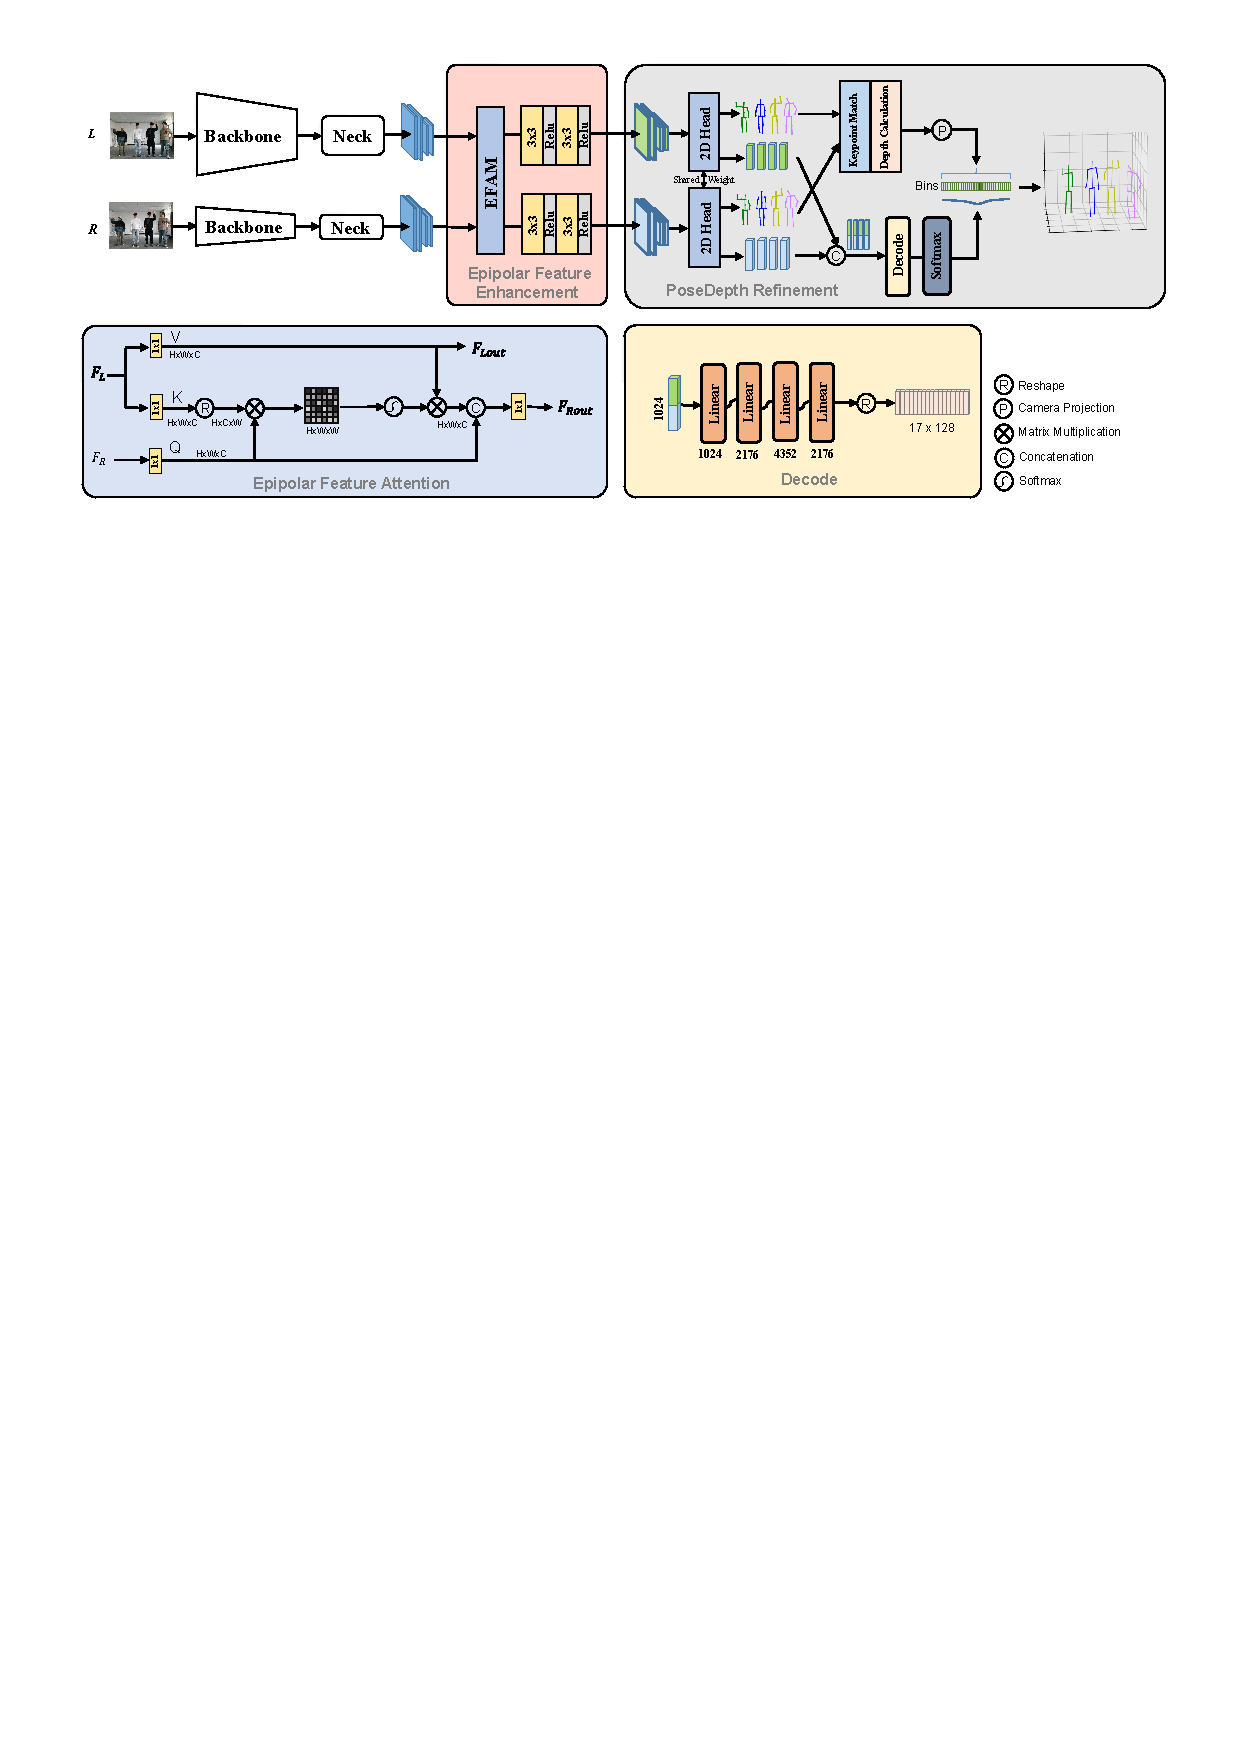
\includegraphics[width=\textwidth]{../figures/pipline.pdf}
\caption{Overview of the StereoMulti3DPose architecture.The model takes left and right stereo images as input and extracts features using asymmetric backbone and neck networks with different model sizes and computational costs. The features are enhanced by the Epipolar Feature Enhancement Module and further refined by the Pose-Depth Refinement module to produce accurate multi-person 3D poses.} \label{models}
\end{figure*}
\subsection{Epipolar Feature Enhancement Module}

To enhance the right-view features using geometric cues from the left view, we propose the Epipolar Feature Enhancement Module (EFEM), which exploits the natural horizontal correspondence in rectified stereo image pairs. In such stereo setups, human keypoints are expected to lie along the same horizontal epipolar lines, which provides a strong prior for feature matching and aggregation across views.

This design is inspired by the idea of leveraging epipolar geometry to guide cross-view feature interaction, as previously explored in the Epipolar Transformer~\citess{he2020epipolar}, which uses attention along the epipolar line to refine 2D pose features. Different from their general multi-view fusion strategy, our method focuses on the stereo setting and explicitly exploits the fixed horizontal correspondence in rectified image pairs for efficient and lightweight attention computation.

Given a left-view feature map \( F_L \in \mathbb{R}^{H \times W \times C} \), we apply a \(1 \times 1\) convolution to project it into key \(K\) and value \(V\) embeddings. Similarly, the right-view feature map \( F_R \) is projected into a query \(Q\).

Since the stereo image pairs are rectified, human keypoints are naturally aligned along the horizontal direction, and this correspondence is further reinforced by the receptive field of the downsampled feature maps. To exploit this property, we reshape \( K \) into \( \tilde{K} \in \mathbb{R}^{H \times C \times W} \), while keeping \( Q \in \mathbb{R}^{H \times W \times C} \), and compute the epipolar attention map:
\begin{equation}
A_{\text{epi}} = \text{Softmax} \left( \frac{Q \tilde{K}}{\sqrt{d}} \right ) \in \mathbb{R}^{H \times W \times W}
\end{equation}
Here, the attention is computed along the horizontal (width) dimension \( W \), enabling each pixel in the right view to attend to all horizontal positions in the left-view feature map. The softmax ensures normalized attention weights across the horizontal line. The attention map is then used to aggregate the left-view values \( V \), producing the enhanced right-view features:
\begin{equation}
\tilde{F}_R = A_{\text{epi}} V
\end{equation}

The enhanced right-view features \( \tilde{F}_R \in \mathbb{R}^{H \times W \times C} \) are concatenated with the original features \( F_R \) along the channel dimension, i.e., \( \hat{F}_R = \text{concat}(F_R, \tilde{F}_R) \in \mathbb{R}^{H \times W \times 2C} \). A \(1 \times 1\) convolution is then applied for feature fusion\citess{hou2025enhanced} and channel reduction, resulting in the output feature map \( F_{Rout} = \text{Conv}_{1 \times 1}(\hat{F}_R) \).

To ensure both branches yield discriminative and high-quality features, we further apply two sequential \(3 \times 3\) convolutions with batch normalization and ReLU activation to the outputs of each branch independently. The final outputs are then forwarded to the detection head for keypoint prediction. This final refinement step enhances local feature representations and strengthens the detection capability of both views.


While the theoretical complexity of the epipolar attention mechanism in EFEM is $O(H \times W^2)$, our design ensures high efficiency for IoT deployment through several strategic optimizations. First, EFEM is applied to downsampled feature maps (e.g., at $1/16$ scale) rather than raw high-resolution inputs. For a standard $640 \times 480$ image, the feature map width $W$ is reduced to 40, making the absolute computational cost of $W^2$ negligible compared to the backbone's heavy convolutions. With a standard channel capacity of $C=128$, the module introduces only about 81.9 K parameters and 0.11 GFLOPs. Second, by exploiting rectified stereo geometry, the attention search is strictly constrained to horizontal scanlines. This pattern aligns with contiguous memory access, facilitating SIMD (Single Instruction, Multiple Data) vectorization on modern IoT processors. Furthermore, for ultra-low-power scenarios, the EFEM provides a flexible optimization path where the search range can be further restricted to a local window $D_{max}$ based on the maximum expected physical disparity. This constraint reduces the practical complexity to $O(H \times W \times D_{max})$ and can be implemented during inference without requiring model retraining, offering a robust method to scale the framework for resource-constrained edge NPUs.

\subsection{PoseDepth Refinement Module}



To enhance the precision and robustness of keypoint-wise depth estimation, especially under the influence of stereo correspondence noise, we propose a poseDepth refinement module that operates within a constrained depth interval $[D - \Delta D, D + \Delta D]$. Here, $D$ denotes the initial depth obtained via triangulation, and $\Delta D$ is a predefined margin that accounts for the uncertainty inherent in stereo matching. By restricting the search space to a local neighborhood around the coarse estimate, we mitigate the risk of large prediction errors while enabling efficient fine-scale refinement.

The depth interval is uniformly discretized into $K$ bins, yielding a quantized set of candidate depths $\{D_1, D_2, \dots, D_K\}$. This discretization transforms the problem into a classification task, which has been empirically shown to offer more stable gradients and better convergence properties compared to direct regression, particularly in scenarios with limited depth annotations.

For each detected person in the image, we extract 2D pose-aware features from both the left and right branches of our network. The features corresponding to the same keypoint from each view are concatenated to form a cross-view joint representation, which captures both local spatial cues and stereo correspondences. Letting $M$ denote the number of detected persons and $J$ the number of keypoints per person, this process yields a total of $M \times J$ fused feature vectors. These are subsequently processed by a lightweight decoder composed of several multilayer perceptrons (MLPs), producing an output tensor of shape $\mathbb{R}^{M \times J \times K}$, where each element represents the logit score for a specific depth bin.

A softmax activation is applied along the depth dimension to produce a discrete probability distribution over depth bins for each keypoint. The final refined depth $\hat{D}_{m,j}$ for the $j$-th keypoint of the $m$-th person is computed as the expectation over the bin centers:

\begin{equation}
\hat{D}_{m,j} = \sum_{i=1}^{K} p_{m,j,i} \cdot D_i,
\end{equation}
where $p_{m,j,i}$ is the normalized probability assigned to the $i$-th bin. This formulation ensures differentiability and allows the model to express uncertainty over nearby depth hypotheses, rather than committing to a single discrete estimate.

To supervise the refinement process, we adopt a Mean Squared Error (MSE) loss between the predicted refined depths and the corresponding ground truth depths:

\begin{equation}
\mathcal{L}_{\text{depth}} = \frac{1}{M J} \sum_{m=1}^{M} \sum_{j=1}^{J} \left( \hat{D}_{m,j} - D^{\text{gt}}_{m,j} \right)^2.
\end{equation}

In all experiments, we fix $\Delta D = 20\,\text{cm}$ and discretize the interval into $K = 128$ uniform bins. This choice reflects a balance between localization precision and computational efficiency. Notably, refining depth individually for each keypoint—rather than searching over the whole 3D space—greatly improves efficiency and supports real-time multi-person performance.

The choice of the search margin $\Delta D = 20 \text{ cm}$ is grounded in both theoretical binocular error analysis and empirical optimization. According to the fundamental geometric triangulation principle~\citess{bracha2021depth, scharstein2002taxonomy}, the depth estimation error $\epsilon_Z$ is quadratically proportional to the distance $Z$ of the observed object:
\begin{equation}
\epsilon_Z \approx \frac{Z^2}{f \cdot B} \epsilon_d
\end{equation}
where $f$ denotes the focal length, $B$ is the baseline, and $\epsilon_d$ represents the disparity matching error. In typical IoT scenarios where baselines are narrow (e.g., $10 \text{ cm}$) and detectors provide only pixel-level accuracy ($\epsilon_d \approx 1\text{--}2 \text{ pixels}$), the theoretical depth uncertainty at an operational range of $3\text{--}8 \text{ meters}$ frequently spans $10\text{--}30 \text{ cm}$~\citess{bracha2021depth}.

Setting $\Delta D = 20 \text{ cm}$ (yielding a $40 \text{ cm}$ total interval) strategically encapsulates these theoretical error bounds. As shown in Table~\ref{The Importance of D}, this value achieved the optimal MPJPE of $51.0 \text{ mm}$. A smaller margin (e.g., $5 \text{ cm}$) fails to cover the initial triangulation noise, while a larger one (e.g., $50 \text{ cm}$) introduces excessive background noise into the bin-classification task, both leading to accuracy degradation. Furthermore, by discretizing this $40 \text{ cm}$ range into $K=128$ uniform bins, our PDRM achieves a fine-grained refinement resolution of approximately $3.1 \text{ mm}$, providing the sub-centimeter precision required for high-fidelity 3D human pose reconstruction.



\subsection{Feature Distillation}

To enhance the feature representation capability of the right branch, we incorporate an online feature distillation mechanism into both the backbone and neck modules. Unlike traditional offline distillation that relies on a fixed teacher network, our approach allows the left (full-scale) and right (lightweight) branches to be trained jointly and simultaneously. The left branch, with its higher capacity and richer representation ability, serves as an adaptive teacher that dynamically provides supervision to the Right branch during training.

This design promotes inter-branch feature alignment and encourages the Right branch to gradually approximate the expressive features learned by the Left branch. In contrast to fixed-teacher paradigms, the online strategy keeps the teacher evolving and more responsive to complex or changing data distributions, which is particularly important in our mixed-domain training setup. Moreover, since both branches share the same input, this structure naturally supports future extensions to mutual learning or consistency-based regularization frameworks.

\begin{figure}[tbp]
    \centering
    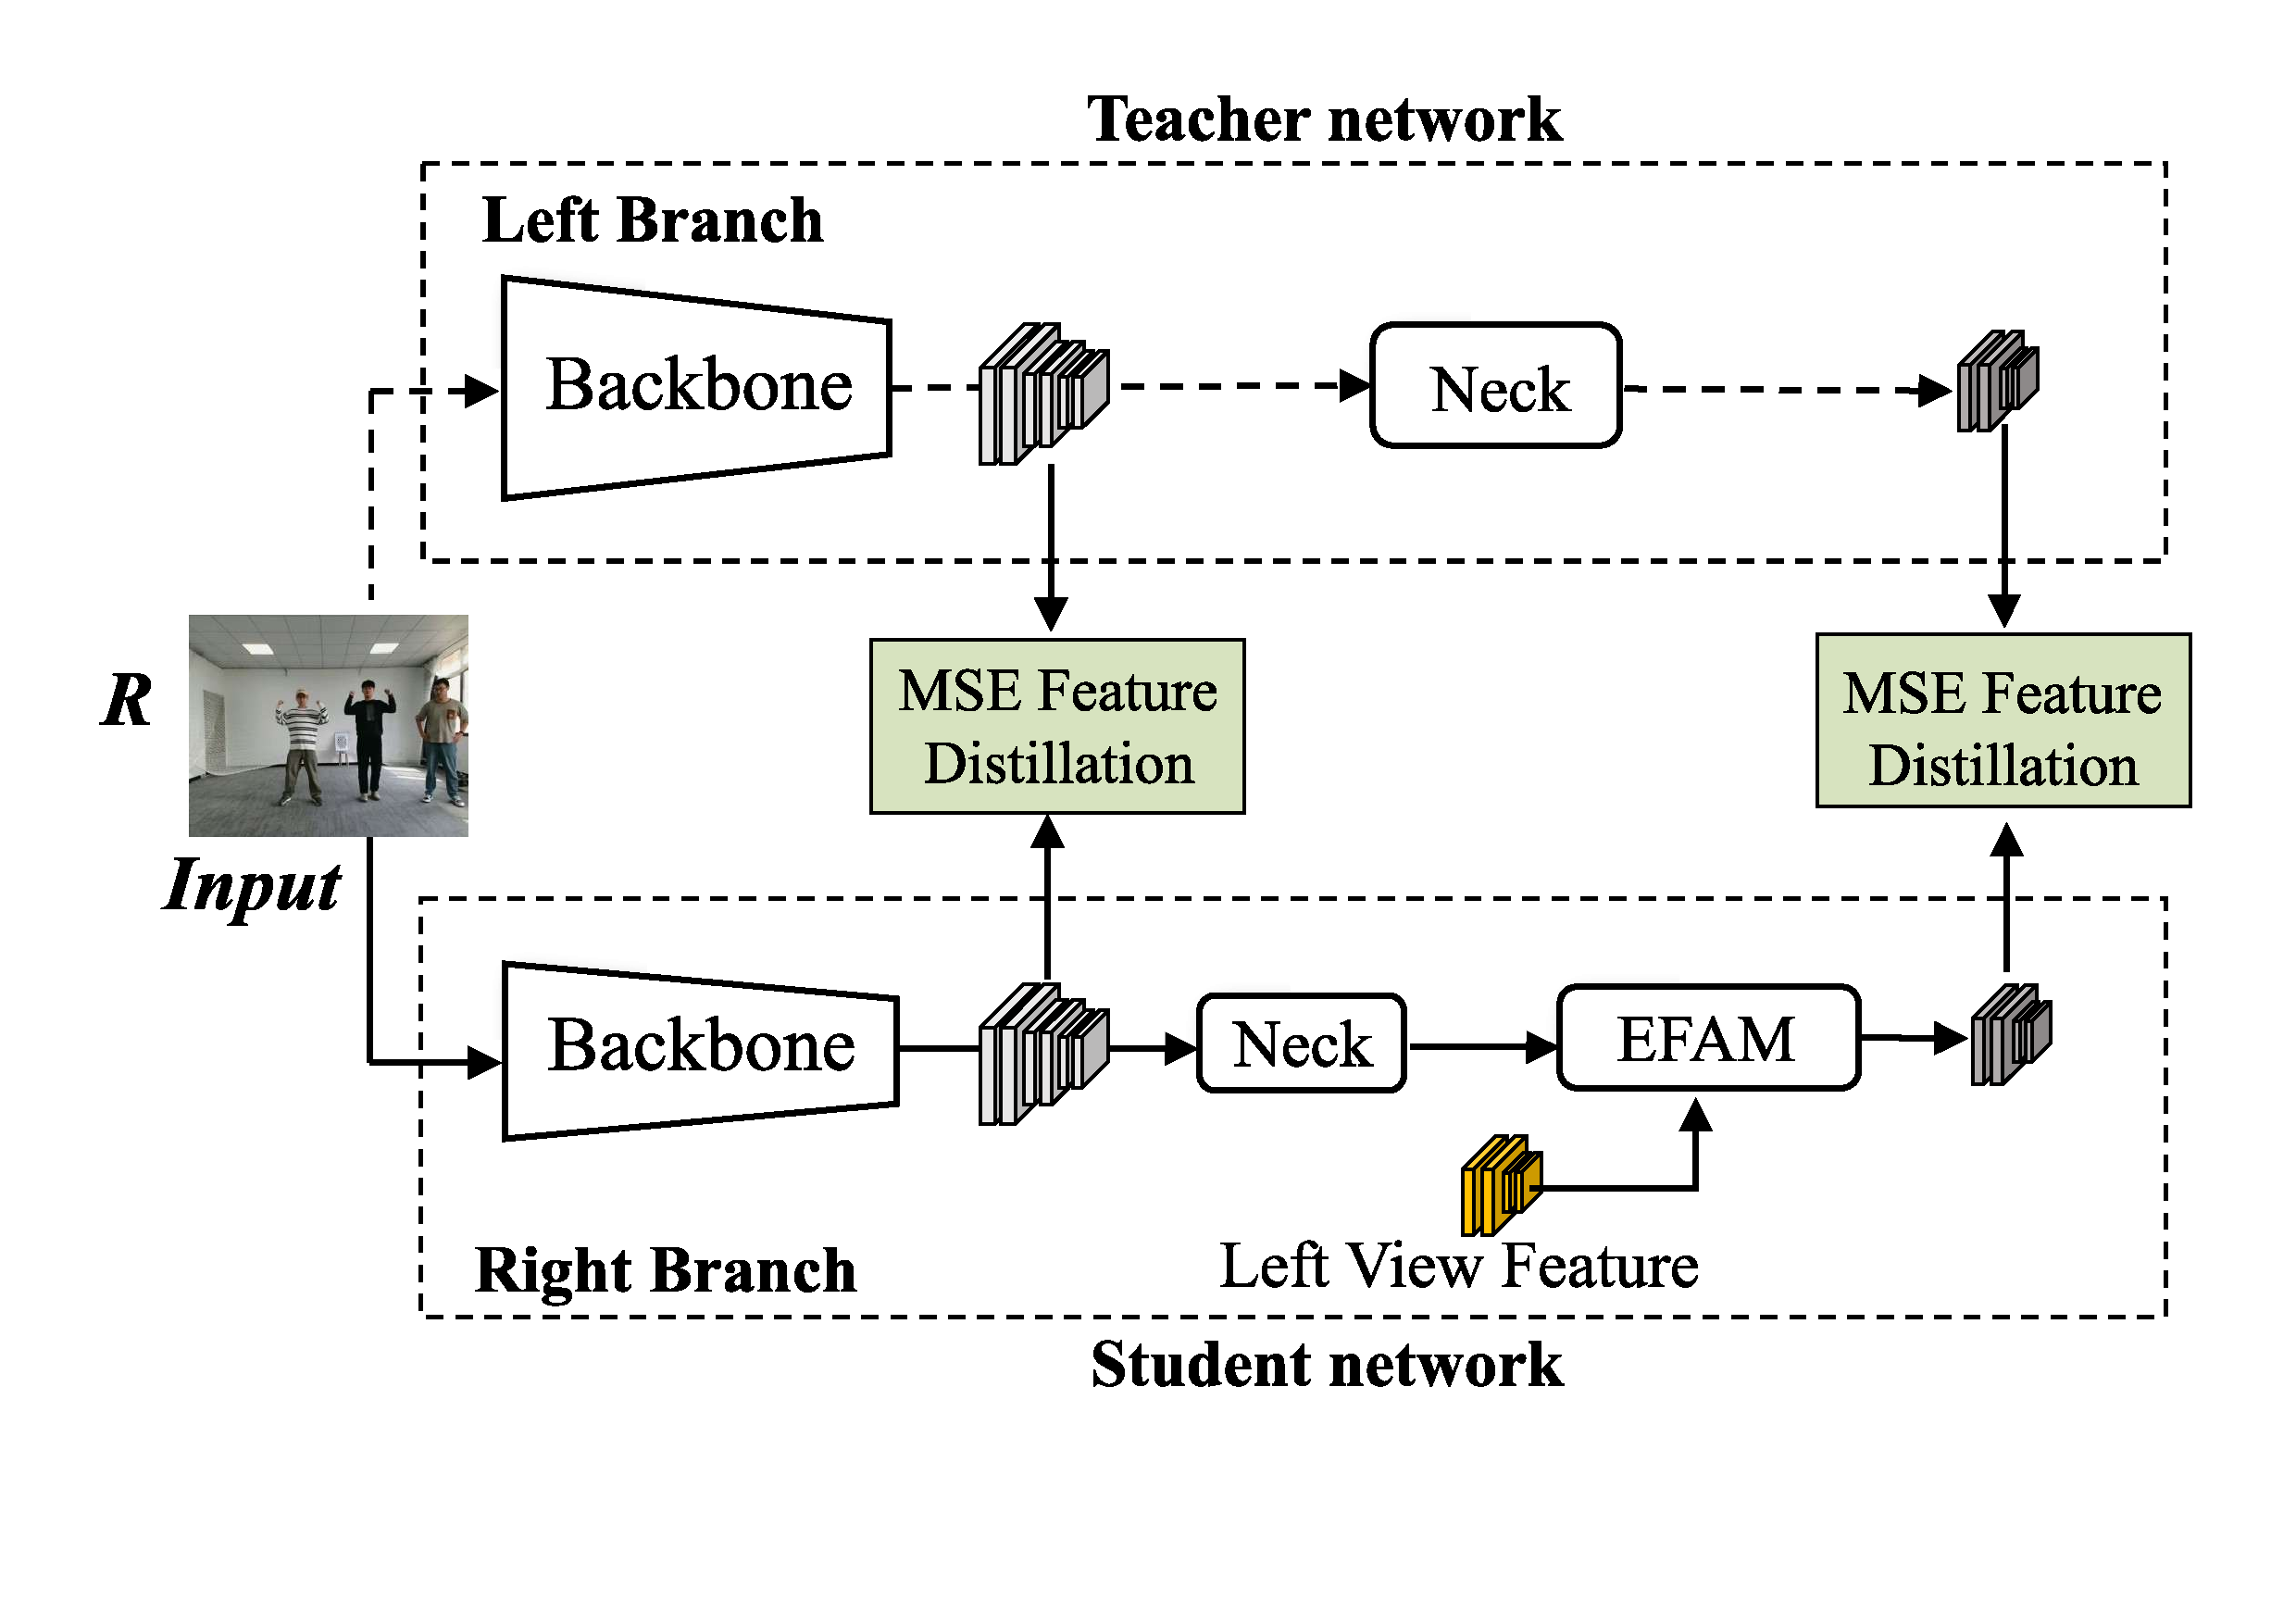
\includegraphics[width=\linewidth]{../figures/dist.pdf}
    \caption{Overview of the online feature distillation framework. During training, both the full-scale Left branch and the lightweight Right branch are jointly optimized. The right-view input passes through both branches, and a distillation loss is applied to intermediate features to encourage the Right branch to mimic the representations of the Left branch.}
    \label{fig:distillation}
\end{figure}

Let \( F_L \) and \( F_R \) denote the feature maps extracted from the Left and Right branches, respectively. To align their representations, we define the feature distillation loss \( \mathcal{L}_{\text{fea}} \) as:

\begin{equation}
\begin{split}
\mathcal{L}_{\text{fea}} = \frac{1}{C \cdot H \cdot W} \sum_{c=1}^{C} \sum_{h=1}^{H} \sum_{w=1}^{W} \Big(
\text{Conv}_{1 \times 1}(F_{L,c,h,w}) \\
- \text{Conv}_{1 \times 1}(F_{R,c,h,w})
\Big)^2
\end{split}
\end{equation}


Here, a \(1 \times 1\) convolution is applied to both branches to ensure the feature dimensions are aligned before computing the mean squared error (MSE) loss. This guides the lightweight branch to learn high-quality feature representations in a supervised yet flexible manner.

The overall training objective combines the 2D keypoint loss, the stereo depth loss, and the feature distillation loss:

\begin{equation}
\mathcal{L} = \lambda_{1} \mathcal{L}_{\text{2d}} + \lambda_{2} \mathcal{L}_{\text{depth}} + \lambda_{3} \mathcal{L}_{\text{fea}}
\end{equation}

where \( \lambda_1, \lambda_2, \lambda_3 \) are the balancing weights for each loss term.





\section{Experiment}

\subsection{Dataset}
Our dataset consists of both synthetic and real-world stereo multi-person pose data, designed to balance diversity and realism.
Following the Human3.6M dataset \citess{ionescu2013human3} , our datasets are annotated with 17 keypoints covering the full human body, ensuring compatibility with existing benchmarks and facilitating performance comparison.
\begin{figure}[!h]
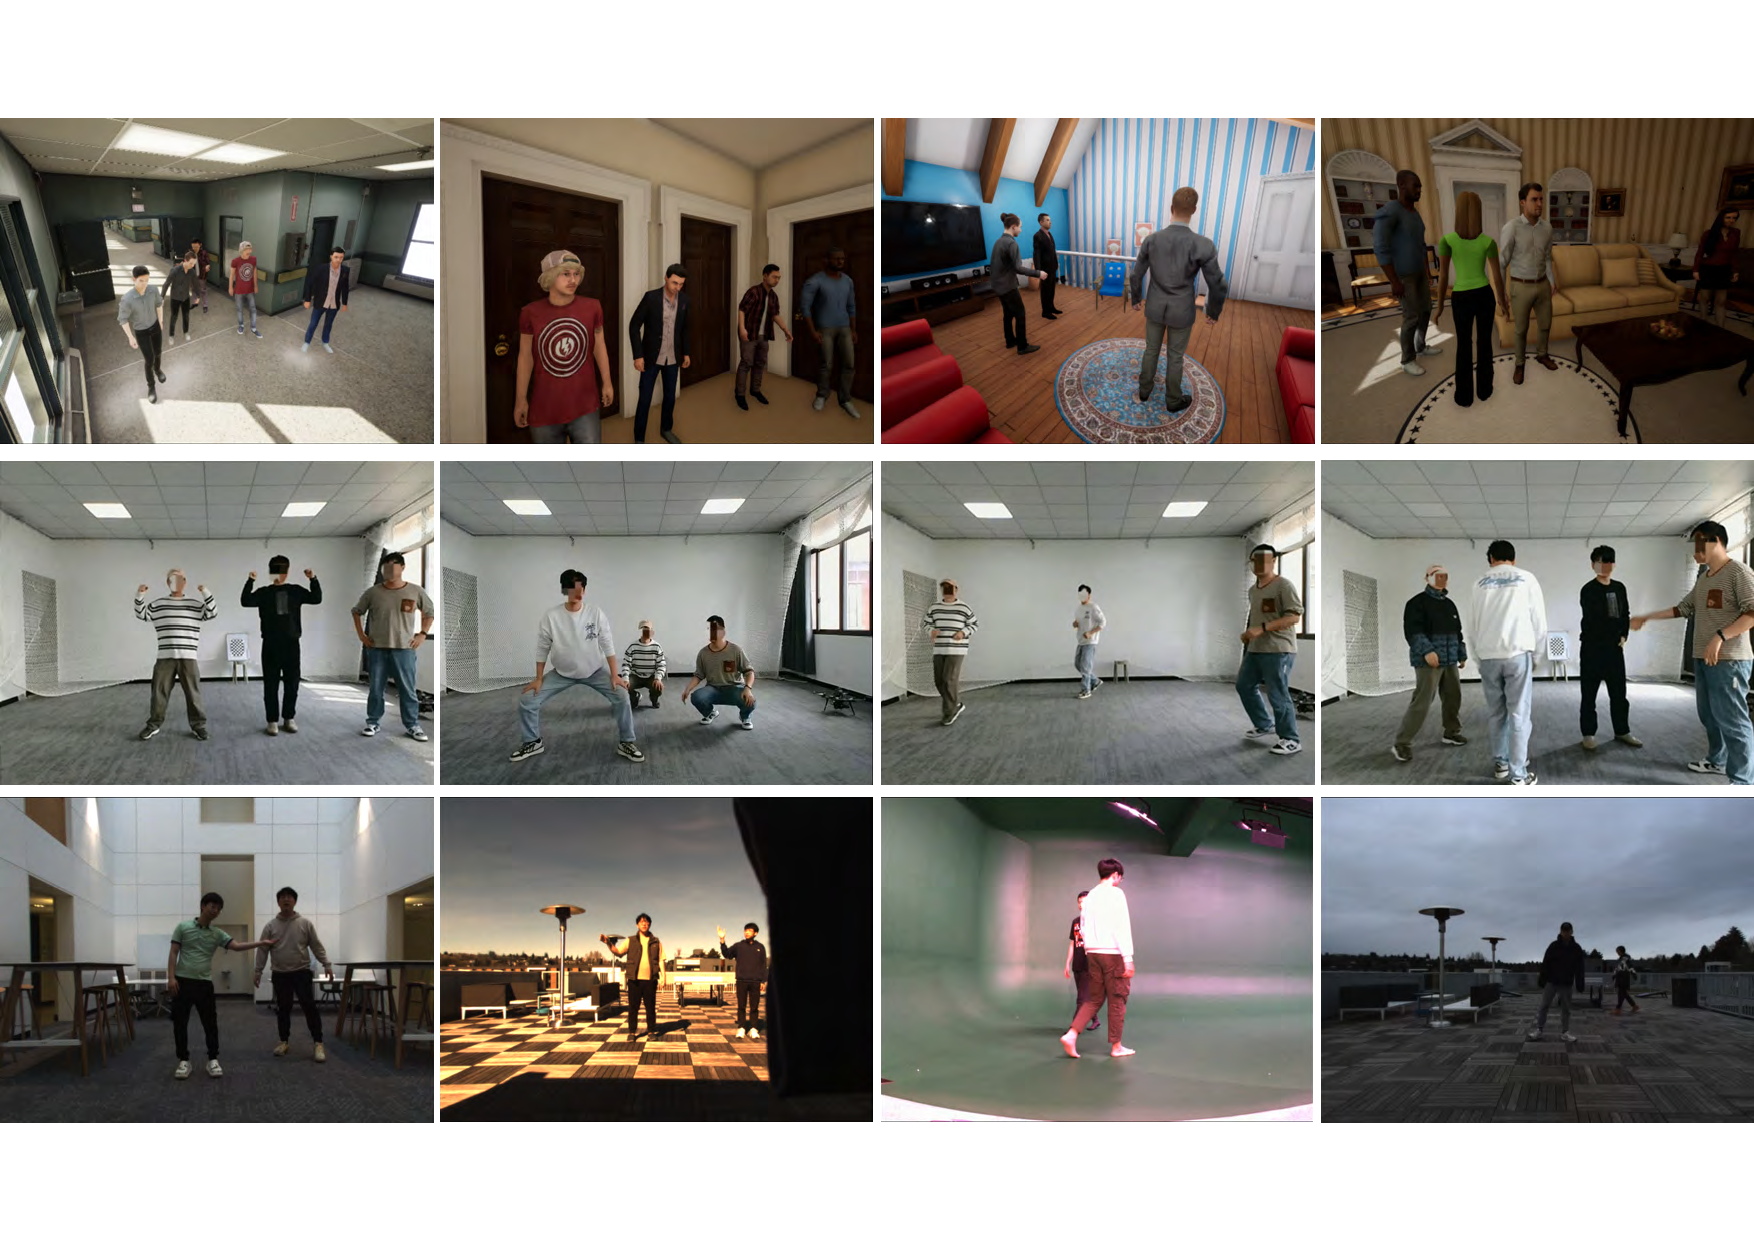
\includegraphics[width=\linewidth]{../figures/dataset-3-crop.pdf}
\caption{Representative samples from the SSMP, BMP, and RT-Pose datasets are shown in the first, second, and third rows, respectively.} \label{dataset}
\end{figure}
\subsubsection{Synthesize Stereo Multi-Person Pose Datasets(SSMP Datasets)}
 Due to the lack of publicly available stereo human pose datasets, we constructed a high-quality stereo multi-person 3D pose dataset using Unreal Engine. This dataset was generated using UnrealCV \citess{qiu2017unrealcv}, simulating real-world camera parameters and lighting conditions with diverse human poses, actions, and backgrounds to improve generalization.
During data generation, we employed precise skeletal animation control and stereo camera simulation of real optical systems to ensure the depth information closely aligns with real-world scenarios. Additionally, to enhance data diversity, we incorporated various human models and clothing variations, making the dataset more robust for training and validating stereo 3D human pose estimation models. The virtual dataset contains a total of 100k raw sample pairs.

\subsubsection{Binocular Multi-Person Pose Dataset(BMP Datasets)}
  We collected a real-world dataset in a laboratory environment, covering various human activities such as sitting, photographing, running, walking, talking, and squatting, following the protocol and action taxonomy of the Human3.6M dataset. To ensure high data accuracy, we leveraged IGEV++ \citess{xu2024igev++} for depth estimation and HRNet \citess{sun2019deep} for 2D pose extraction, both of which are state-of-the-art (SOTA) methods in their respective fields. This dataset is designed for evaluating and optimizing our model’s performance in real-world scenarios and contains a total of 20k samples.
\subsubsection{RT-Pose Dataset}
To better evaluate the model in complex real-world scenarios, we employ the RT-Pose Dataset \citess{ho2024rt} as a benchmark. RT-Pose consists of 4D radar tensors, LiDAR point clouds, and RGB images, comprising 72k frames across 240 sequences and covering six types of human actions with different complexity levels. The annotations are generated through the joint calibration of RGB images and LiDAR, resulting in accurate 3D skeleton labels. Compared to datasets that rely solely on RGB, RT-Pose better reflects the challenges of complex real-world scenarios and provides a reliable benchmark for evaluating model robustness and generalization. In our experiments, we use only the stereo RGB images from RT-Pose as input for training and evaluation.
\begin{table*}[!ht]
\caption{We compared our method with existing approaches on a real-world dataset and evaluated the average inference time on the test set. For the dual-branch prediction model, the number of parameters and computational cost are doubled compared to the original. The symbol * indicates our re-implementation.}\label{benchmark}
\centering
\resizebox{\textwidth}{!}{
\begin{tabular}{|c|cccclcc|c|c|ccc|}

\hline

\multicolumn{1}{|c|}{\multirow{2}{*}{Method}} & \multicolumn{7}{c|}{MPJPE(mm)}                                                                                                                                                                                                                                   & \multicolumn{1}{c|}{\multirow{2}{*}{Param}} & \multirow{2}{*}{Flops} \\ \cline{2-8}
\multicolumn{1}{|c|}{}                        & \multicolumn{1}{c|}{Waving}         & \multicolumn{1}{c|}{Walking}          & \multicolumn{1}{c|}{Sitting}       & \multicolumn{1}{c|}{Talking}       & \multicolumn{1}{c|}{Taking photos}         & \multicolumn{1}{c|}{Squatting}     & \multicolumn{1}{c|}{Avg}           & \multicolumn{1}{c|}{}                       &                        \\ \hline
\multicolumn{10}{|c|}{Monocular Method}                                                                                                                                                                                                                                                                                                                                                 \\ \hline
\multicolumn{1}{|c|}{Simple Baseline\citess{martinez2017simple}}         & \multicolumn{1}{c|}{123.4}         & \multicolumn{1}{c|}{132.1}         & \multicolumn{1}{c|}{154.7}         & \multicolumn{1}{c|}{127.5}         & \multicolumn{1}{c|}{132.0}         & \multicolumn{1}{c|}{182.6}         & \multicolumn{1}{c|}{142.1}         & \multicolumn{1}{c|}{23.48M}                 & 67.19G                 \\
\multicolumn{1}{|c|}{JointFormer\citess{lutz2022jointformer}}             & \multicolumn{1}{c|}{102.9}         & \multicolumn{1}{c|}{123.3}         & \multicolumn{1}{c|}{143.3}         & \multicolumn{1}{c|}{112.8}         & \multicolumn{1}{c|}{121.4}         & \multicolumn{1}{c|}{173.0}         & \multicolumn{1}{c|}{129.5}         & \multicolumn{1}{c|}{48.61M}                 & 160.66G                \\
\multicolumn{1}{|c|}{RTMW3D\citess{jiang2024rtmw}}                  & \multicolumn{1}{c|}{92.2}          & \multicolumn{1}{c|}{114.6}         & \multicolumn{1}{c|}{132.3}         & \multicolumn{1}{c|}{110.9}         & \multicolumn{1}{c|}{112.1}         & \multicolumn{1}{c|}{144.3}         & \multicolumn{1}{c|}{117.7}         & \multicolumn{1}{c|}{92.30M}                 & 136.56G                \\ \hline
\multicolumn{10}{|c|}{Two-Stage Method} \\ \hline
\multicolumn{1}{|c|}{MobiDepthPose\citess{zhang2022mobidepth}}           & \multicolumn{1}{c|}{173.2}         & \multicolumn{1}{c|}{184.3}         & \multicolumn{1}{c|}{193.2}         & \multicolumn{1}{c|}{181.4}         & \multicolumn{1}{c|}{183.2}         & \multicolumn{1}{c|}{223.3}         & \multicolumn{1}{c|}{189.8}         & \multicolumn{1}{c|}{7.27M}                  & 10.36G                 \\
\multicolumn{1}{|c|}{RTMO\citess{lu2024rtmo}+SGBM\citess{hirschmuller2005accurate}}               & \multicolumn{1}{c|}{93.3}          & \multicolumn{1}{c|}{103.4}         & \multicolumn{1}{c|}{119.0}         & \multicolumn{1}{c|}{121.8}         & \multicolumn{1}{c|}{117.9}         & \multicolumn{1}{c|}{134.2}         & \multicolumn{1}{c|}{114.9}         & \multicolumn{1}{c|}{9.8M}                   & 12.13G                 \\
\multicolumn{1}{|c|}{RTMO\citess{lu2024rtmo}+MobileStereoNet\citess{shamsafar2022mobilestereonet}}    & \multicolumn{1}{c|}{72.9}          & \multicolumn{1}{c|}{79.1}          & \multicolumn{1}{c|}{103.6}         & \multicolumn{1}{c|}{97.2}          & \multicolumn{1}{c|}{83.4}          & \multicolumn{1}{c|}{103.2}         & \multicolumn{1}{c|}{89.9}          & \multicolumn{1}{c|}{12.09M}                 & 116.12G                \\ \hline
\multicolumn{10}{|c|}{Dual Branch Method}                                                                                                                                                                                                                                                                                                                                               \\ \hline
\multicolumn{1}{|c|}{Dual Yolo-Pose\citess{maji2022yolo}}          & \multicolumn{1}{c|}{171.6}         & \multicolumn{1}{c|}{172.3}         & \multicolumn{1}{c|}{189.7}         & \multicolumn{1}{c|}{172.9}         & \multicolumn{1}{c|}{189.3}         & \multicolumn{1}{c|}{219.5}         & \multicolumn{1}{c|}{185.9}         & \multicolumn{1}{c|}{9.9M}                   & 46.4G                  \\
\multicolumn{1}{|c|}{Dual RTMO\citess{lu2024rtmo}}               & \multicolumn{1}{c|}{110.6}         & \multicolumn{1}{c|}{123.0}         & \multicolumn{1}{c|}{172.6}         & \multicolumn{1}{c|}{141.1}         & \multicolumn{1}{c|}{163.9}         & \multicolumn{1}{c|}{182.4}         & \multicolumn{1}{c|}{148.9}         & \multicolumn{1}{c|}{9.869M}                 & 24.25G                 \\ \hline
\multicolumn{10}{|c|}{End to End Method} \\ \hline
DMCPose*~\citess{10908018}                                  & \multicolumn{1}{c|}{53.2} & \multicolumn{1}{c|}{58.4} & \multicolumn{1}{c|}{71.8} & \multicolumn{1}{c|}{56.8} & \multicolumn{1}{c|}{63.8} & \multicolumn{1}{c|}{81.9} & \multicolumn{1}{c|}{64.3}   & \multicolumn{1}{c|}{27.1M}                 & 41.1G \\ \hline
\textbf{Ours}           & \multicolumn{1}{c|}{\textbf{39.1}} & \multicolumn{1}{c|}{\textbf{41.6}} & \multicolumn{1}{c|}{\textbf{59.9}} & \multicolumn{1}{c|}{\textbf{42.8}} & \multicolumn{1}{c|}{\textbf{52.4}} & \multicolumn{1}{c|}{\textbf{70.1}} & \multicolumn{1}{c|}{\textbf{51.0}} & \multicolumn{1}{c|}{11.7M}                  & 13.93G                 \\ \hline
\end{tabular}
}
\end{table*}





\subsection{Implementation Details}
To mitigate the sim-to-real gap, our framework incorporates several techniques beyond standard fine-tuning~\citess{peng2018sim, mueller2018ganerated}. . First, we employed extensive Domain Randomization during synthetic data generation in Unreal Engine, simulating diverse lighting, backgrounds, and real-world camera parameters to force the model to prioritize geometric structures over synthetic textures. Second, we utilized explicit geometric normalization via epipolar rectification for all real-world samples. This ensures that the universal physical laws of binocular vision—which the EFEM module exploits through 1D scanline searches—remain consistent across both virtual and real domains. We use an 80-10-10 split, with 80\% for training, 10\% for validation, and 10\% for testing. The 80-10-10 data split for the SSMP dataset is justified by its large-scale nature (100,000 samples), where the 10,000-sample test set ensures reliable performance evaluation without the need for computationally expensive cross-validation. Furthermore, as a domain-specific consideration, this split supports our two-stage Sim-to-Real pipeline, ensuring that the model learns robust geometric feature representations during pre-training before fine-tuning on real-world scenarios. This methodology optimizes the trade-off between training convergence stability and computational efficiency, fulfilling the requirements for IoT-oriented research. The left branch adopts a YOLO-style architecture with CSPDarknet \citess{bochkovskiy2020yolov4} for accurate 2D keypoint detection, while the right branch employs ShuffleNetV2 \citess{ma2018shufflenet} and Lightweight FPN \citess{E210226} for efficient multi-scale feature extraction.

In the first stage, the model is pretrained on the SSMP Datasets. Following the standard practice in stereo vision \citess{Godard_2017_CVPR}, we implement a symmetric data augmentation strategy to ensure the model learns intrinsic geometric constraints rather than branch-specific features. In addition to random color transformations and cropping, we specifically incorporate on-the-fly horizontal flipping combined with left-right view swapping. This procedure ensures that the Epipolar Feature Enhancement Module (EFEM) encounters both (Left-Full/Right-Compact) and (Right-Full/Left-Compact) configurations during training, forcing it to attend to horizontal correspondences along epipolar lines. The input images are resized to 480×640, and data augmentation techniques, including random color transformations (hue, saturation, contrast), brightness adjustment, random cropping, and mean-variance normalization, are applied, following the training pipeline of MMPose \citess{mmpose2020}. The learning rate is set to $5\times10^{-3}$, with a distillation loss weight decay factor of $0.0002$, and the model is trained for 500 epochs. The weighting hyperparameters in the multi-task loss function are set as: $\lambda_{1} = 5, \lambda_{2} = 5, \lambda_{3} = 1$. In the second stage, fine-tuning is conducted on the BMP Datasets with the distillation loss removed, and the learning rate adjusted to $2\times10^{-4}$. The model is trained for 100 epochs, and real data undergoes epipolar rectification before being fed into the network to ensure geometric consistency between stereo image pairs. All experiments are conducted on a Linux system using a single NVIDIA L40s GPU. The model is implemented within the MMPose framework and trained with PyTorch using a batch size of 128.
\subsection{Evaluation metrics}
We use a common evaluation metric, \textbf{Mean Per Joint Position Error (MPJPE)}, to measure the accuracy of 3D human pose estimation. MPJPE calculates the average Euclidean distance between the predicted and ground-truth joint coordinates across all samples and joints:

\begin{equation}
\text{MPJPE} = \frac{1}{N \times J} \sum_{i=1}^{N} \sum_{j=1}^{J} \left\| \hat{\mathbf{P}}_{i,j} - \mathbf{P}_{i,j} \right\|_2
\end{equation}

Here, \( N \) denotes the number of samples, and \( J \) is the number of 3D joints per sample.
\( \hat{\mathbf{P}}_{i,j} \in \mathbb{R}^3 \) and \( \mathbf{P}_{i,j} \in \mathbb{R}^3 \) represent the predicted and ground-truth 3D positions of the \( j \)-th joint in the \( i \)-th sample, respectively.
\( \left\| \cdot \right\|_2 \) denotes the Euclidean norm.



\begin{table*}[!ht]
\caption{We compared our method with existing approaches on RT-Pose dataset, both indoor and outdoor test-sets.}\label{benchmark2}
\centering
\resizebox{0.8\textwidth}{!}{
\begin{tabular}{|c|cccccc|}
\hline
\multicolumn{1}{|c|}{\multirow{2}{*}{Method}} & \multicolumn{6}{c|}{MPJPE(mm)} \\ \cline{2-7}
\multicolumn{1}{|c|}{}                        & \multicolumn{1}{c|}{Waving Hand} & \multicolumn{1}{c|}{Lifting Leg} & \multicolumn{1}{c|}{Random Pose} & \multicolumn{1}{c|}{Normal} & \multicolumn{1}{c|}{Sitting}  & \multicolumn{1}{c|}{Avg} \\ \hline

\multicolumn{7}{|c|}{Monocular Method} \\ \hline
Simple Baseline\citess{martinez2017simple}          & \multicolumn{1}{c|}{353.2} & \multicolumn{1}{c|}{342.1} & \multicolumn{1}{c|}{362.6} & \multicolumn{1}{c|}{422.1} & \multicolumn{1}{c|}{391.8} & \multicolumn{1}{c|}{374.3} \\ \hline
JointFormer\citess{lutz2022jointformer}            & \multicolumn{1}{c|}{332.1} & \multicolumn{1}{c|}{312.8} & \multicolumn{1}{c|}{342.1} & \multicolumn{1}{c|}{369.5} & \multicolumn{1}{c|}{329.8} & \multicolumn{1}{c|}{337.2} \\
RTMW3D\citess{jiang2024rtmw}                      & \multicolumn{1}{c|}{298.3}  & \multicolumn{1}{c|}{292.8} & \multicolumn{1}{c|}{327.4} & \multicolumn{1}{c|}{331.2} & \multicolumn{1}{c|}{287.0} & \multicolumn{1}{c|}{307.3} \\ \hline

\multicolumn{7}{|c|}{Two-Stage Method} \\ \hline
MobiDepthPose\citess{zhang2022mobidepth}                         & \multicolumn{1}{c|}{221.3} & \multicolumn{1}{c|}{215.7} & \multicolumn{1}{c|}{207.5} & \multicolumn{1}{c|}{208.9} & \multicolumn{1}{c|}{223.3} & \multicolumn{1}{c|}{215.3}  \\
RTMO\citess{lu2024rtmo}+SGBM\citess{hirschmuller2005accurate}      & \multicolumn{1}{c|}{205.0}  & \multicolumn{1}{c|}{208.0} & \multicolumn{1}{c|}{219.7} & \multicolumn{1}{c|}{224.6} & \multicolumn{1}{c|}{202.4} & \multicolumn{1}{c|}{211.9} \\
RTMO\citess{lu2024rtmo}+MobileStereoNet\citess{shamsafar2022mobilestereonet} & \multicolumn{1}{c|}{193.6} & \multicolumn{1}{c|}{187.3} & \multicolumn{1}{c|}{208.9} & \multicolumn{1}{c|}{219.6} & \multicolumn{1}{c|}{ 200.5} & \multicolumn{1}{c|}{202.0}  \\ \hline

\multicolumn{7}{|c|}{Dual Branch Method} \\ \hline
Dual Yolo-Pose\citess{maji2022yolo}          & \multicolumn{1}{c|}{261.3} & \multicolumn{1}{c|}{256.8} & \multicolumn{1}{c|}{269.7} & \multicolumn{1}{c|}{258.4} & \multicolumn{1}{c|}{233.1} & \multicolumn{1}{c|}{255.8} \\
Dual RTMO\citess{lu2024rtmo}                       & \multicolumn{1}{c|}{241.9} & \multicolumn{1}{c|}{238.7} & \multicolumn{1}{c|}{245.6} & \multicolumn{1}{c|}{256.9} & \multicolumn{1}{c|}{228.1} & \multicolumn{1}{c|}{242.2} \\ \hline
\multicolumn{7}{|c|}{End to End Method} \\ \hline
DMCPose*\citess{10908018}                                   & \multicolumn{1}{c|}{187.9} & \multicolumn{1}{c|}{189.3} & \multicolumn{1}{c|}{195.7} & \multicolumn{1}{c|}{209.8} & \multicolumn{1}{c|}{201.4}  & \multicolumn{1}{c|}{196.8} \\ \hline
    \textbf{Ours}                                   & \multicolumn{1}{c|}{\textbf{162.3}} & \multicolumn{1}{c|}{\textbf{156.9}} & \multicolumn{1}{c|}{\textbf{163.9}} & \multicolumn{1}{c|}{\textbf{177.4}} & \multicolumn{1}{c|}{\textbf{132.6}} & \multicolumn{1}{c|}{\textbf{158.6}} \\ \hline
\end{tabular}
}
\end{table*}
\subsection{Benchmark}

For monocular methods (i.e., SimpleBaseline \citess{martinez2017simple}, JointFormer \citess{lutz2022jointformer}, and RTMW3D \citess{jiang2024rtmw}), we fine-tune the models on our dataset prior to evaluation to ensure a fair comparison. To enhance reproducibility, we adopt a unified training configuration across baselines: the learning rate is set to $1\times10^{-4}$ for SimpleBaseline and JointFormer, and to $2\times10^{-3}$ for RTMW3D. The batch size is fixed at 64, and all models are optimized using Adam with a weight decay of $1\times10^{-4}$, trained for 100 epochs.

For the two-stage method (i.e., MobiDepthPose \citess{zhang2022mobidepth}), we directly employ the pretrained weights without further fine-tuning. For RTMO \citess{lu2024rtmo}+SGBM \citess{hirschmuller2005accurate}, we use RTMO-s and set $\text{minDisparity}=0$ and $\text{numDisparities}=192$ for SGBM. For RTMO \citess{lu2024rtmo}+MobileStereoNet \citess{shamsafar2022mobilestereonet}, we also use the RTMO-s model and set $\text{numDisparities}=192$ for MobileStereoNet.

For dual-branch methods (i.e., Dual Yolo-Pose \citess{maji2022yolo} and Dual RTMO \citess{lu2024rtmo}), we first employ their respective 2D detectors (Yolo-Pose and RTMO) to localize 2D keypoints independently in the left and right images, and then reconstruct 3D poses via triangulation. Dual Yolo-Pose adopts the Yolo-Pose-s model, which uses CSP-Darknet53 \citess{bochkovskiy2020yolov4} as the backbone and PANet \citess{wang2019panet} for multi-scale feature fusion. Dual RTMO employs the RTMO-s model with CSP-Darknet53 as the backbone, while further enhancing the last three feature maps using a Hybrid Encoder \citess{zhao2024detrs}.

For end-to-end methods (i.e., DMCPose \citess{10908018}), we reproduced the model based on the descriptions provided in the original paper, as no official implementation was publicly available. Our reproduction employs a ResNet-50 \citess{he2016deep} backbone and follows the same loss functions and training strategies reported in the original work to ensure a fair comparison.
\subsection{Result}
A comprehensive comparison is provided in Table~\ref{benchmark}. Compared to existing methods, our approach shows significant advantages across simple and complex scenes. Monocular methods perform well in simple scenarios like Waving and Walking, but suffer in complex ones like Sitting and Squatting; RTMW3D achieves an average error of 117.7cm, which is approximately 56.6\% higher than our method's error. Two-stage methods like RTMO+MobileStereoNet reduce errors in simple scenes but struggle in complex scenarios, such as Sitting, with an error of 103.6 cm. Notably, MobileStereoNet has a high computational cost, with 116.12G FLOPs. In contrast, our method achieves 59.9cm in Sitting and 70.1cm in Squatting, while maintaining a much lower computational cost of 13.93G FLOPs. Dual-branch methods have high errors in complex scenes (e.g., 163.9cm in Photo), while our methods enhances stereo feature representation, achieving 51.0cm in overall accuracy.
\begin{figure}[!htb]
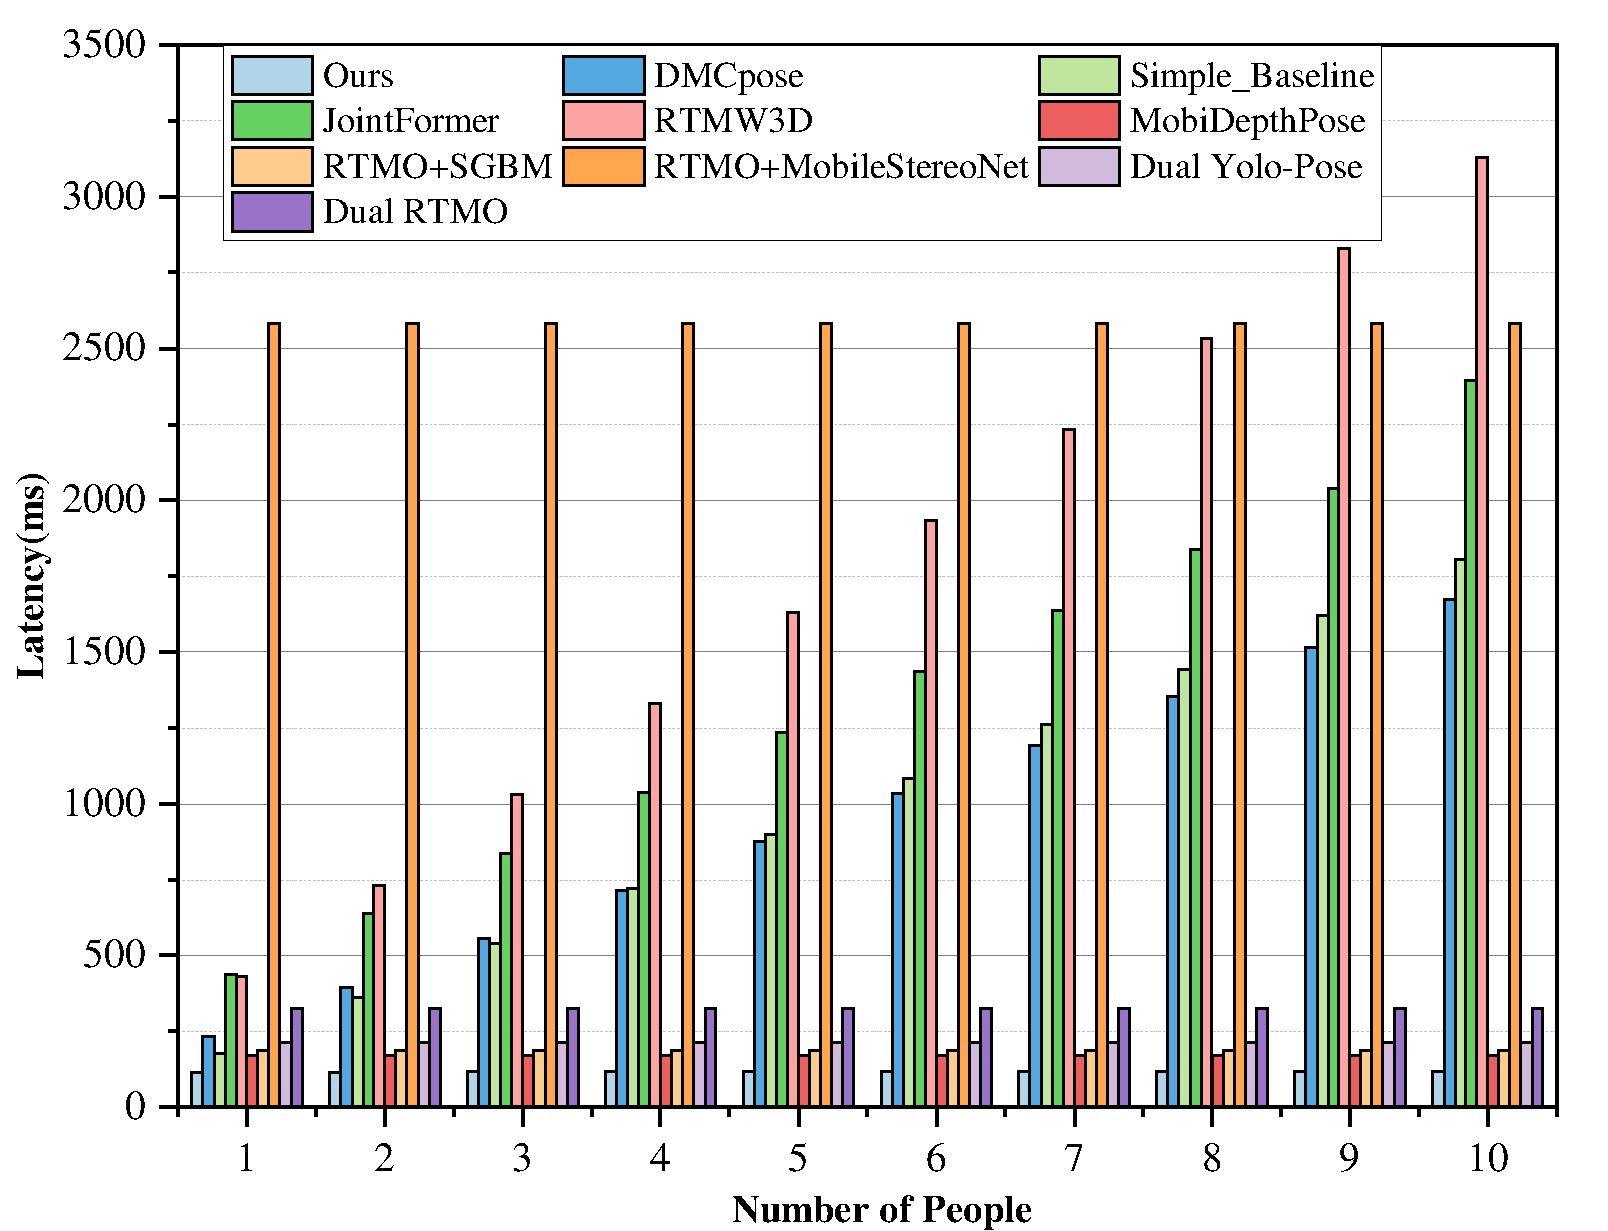
\includegraphics[width=\linewidth]{../figures/latency.pdf}
\caption{The variation in inference latency with respect to the number of people, ranging from 1 to 10. } \label{fig1}
\end{figure}


To evaluate StereoMulti3DPose in challenging situations, we tested it on the RT-Pose Datasets benchmark. The results are summarized Table~\ref{benchmark2}. Our model is more robust under different actions under complex indoor and outdoor environments. For example, in the Random Pose scenario, our model achieves an MPJPE of 163.9 mm, whereas the stereo-based Dual Yolo-Pose reports an error of 269.7 mm. In summary, our method outperforms existing approaches in both accuracy and computational efficiency.

\begin{table}[h]
    \centering
    \small
    \caption{Cross-platform hardware performance and energy stability. The latency is measured for a single subject to represent the baseline inference speed. The average power increase represents the delta between active inference and idle state.}
    \label{tab:hardware_efficiency_simplified}
    \renewcommand{\arraystretch}{1.5}
    \resizebox{\linewidth}{!}{
        \begin{tabular}{lccccc}
            \hline
            \textbf{Hardware Platform} & \textbf{Processor} & \textbf{Engine} & \textbf{Precision} & \textbf{Latency (ms)} & \textbf{Avg. Power Increase} \\
            & & & & (1 Person) & \textbf{(Active vs. Idle)} \\ \hline

            NVIDIA Jetson AGX Xavier &  GPU & TensorRT & FP16 & 25.3 & + 13.5 W \\ \hline
            Origin Pi RK3588 &  NPU & RKNN & INT8 & 89.0 & + 2.1 W \\ \hline
            Raspberry Pi 4B &  CPU & MNN & FP32 & 210.5 & + 3.8 W \\ \hline
        \end{tabular}
    }
\end{table}


To evaluate the deployment potential of StereoMulti3DPose across diverse IoT ecosystems, we benchmarked its performance on three representative hardware architectures (Table\ref{tab:hardware_efficiency_simplified}). The results demonstrate that the framework achieves high-speed inference across all platforms. The NVIDIA Jetson AGX Xavier establishes a high-performance baseline of 25.3 ms by leveraging its Volta GPU and TensorRT optimization. On the specialized AIoT platform, Origin Pi RK3588, the integrated 6 TOPS NPU utilizes INT8 quantization to deliver a balanced latency of 89.0 ms with an exceptionally low power increase of only +2.1W, highlighting its superior energy efficiency for power-constrained edge nodes. Even on the general-purpose Raspberry Pi 4B, the model remains functional with manageable power fluctuations.


Additionally, we conduct a quantitative analysis of inference performance on IoT platforms and evaluated the latency for multi-person scenarios involving 1 to 10 individuals, as shown in Fig.~\ref{fig1}. The top-down method uses MMDetection\citess{mmdetection}. During inference, input images are resized to 640×480, and the MNN\citess{jiang2020mnn} inference engine is used with the ARMv8.2 instruction set and FP16 data format. CPU inference latency is measured in a 4-thread mode. To ensure a rigorous and fair comparison, all latency results were obtained using an identical hardware environment, specifically a Xiaomi 14 smartphone equipped with a Snapdragon 8 Gen3 processor and 16GB of RAM. To guarantee statistical reliability, the reported values represent the average inference time calculated across the entire test set using the MNN engine in a 4-thread FP16 configuration, thereby mitigating the impact of transient system fluctuations.

The results show that StereoMulti3DPose, based on 2D multi-person pose estimation, offers advantages in multi-person scenarios. Although the latency of the 3D head increases with the number of individuals, its overall contribution to the total inference time remains minimal. For example, in scenarios with 8-10 individuals, the 3D head accounts for only 1\% of the total inference time.
\begin{table}[htbp]
\centering
\caption{Detailed latency profiling of StereoMulti3DPose on Xiaomi 14. The 3D head (PDRM) exhibits minimal incremental cost despite scaling person count or resolution.}
\label{latency_profiling}
\resizebox{\linewidth}{!}{
\begin{tabular}{lcccc}
\hline
\textbf{Configuration} & \textbf{Resolution} & \textbf{Total (ms)} & \textbf{3D Head (ms)} & \textbf{Inc. Latency} \\ \hline
\textit{Person Count Variation} & & & & \\ \hline
1 Person & 640$\times$480 & 116.0 & 10.2 & Baseline \\ \hline
10 People & 640$\times$480 & 117.3 & 12.5 & \textbf{1.1\%} \\ \hline \hline
\textit{Resolution Variation} & & & & \\ \hline
Low-Res & 320$\times$320 & 58.5 & 12.5 & 4.3\% \\ \hline
Standard & 640$\times$480 & 117.3 & 12.5 & 2.1\% \\ \hline
High-Res & 1280$\times$720 & 486.2 & 12.5 & 0.5\% \\ \hline
\end{tabular}
}
\end{table}

To evaluate the scalability of StereoMulti3DPose for real-time IoT sensing, we provide a detailed profiling of inference latency on the Xiaomi 14 platform. As demonstrated in Table~\ref{latency_profiling}, our framework maintains a remarkably stable performance regardless of the scene complexity. Specifically, when the number of people increases from 1 to 10, the total latency only experiences an incremental increase of approximately 1.1\%. This is because the PDRM (3D head) operates on sparse M×J feature vectors rather than performing dense convolutions, ensuring the system maintains a nearly constant latency of 116 ms per stereo pair. Furthermore, while the total latency scales with the image resolution due to the backbone's workload, the absolute execution time of the 3D head remains constant at 12.5 ms, confirming its computational decoupling from the pixel scale. Since IoT devices typically process live video streams with a Batch Size of 1, this architecture is ideal for consistent, real-time 3D perception in crowded environments.

\begin{figure}[!h]

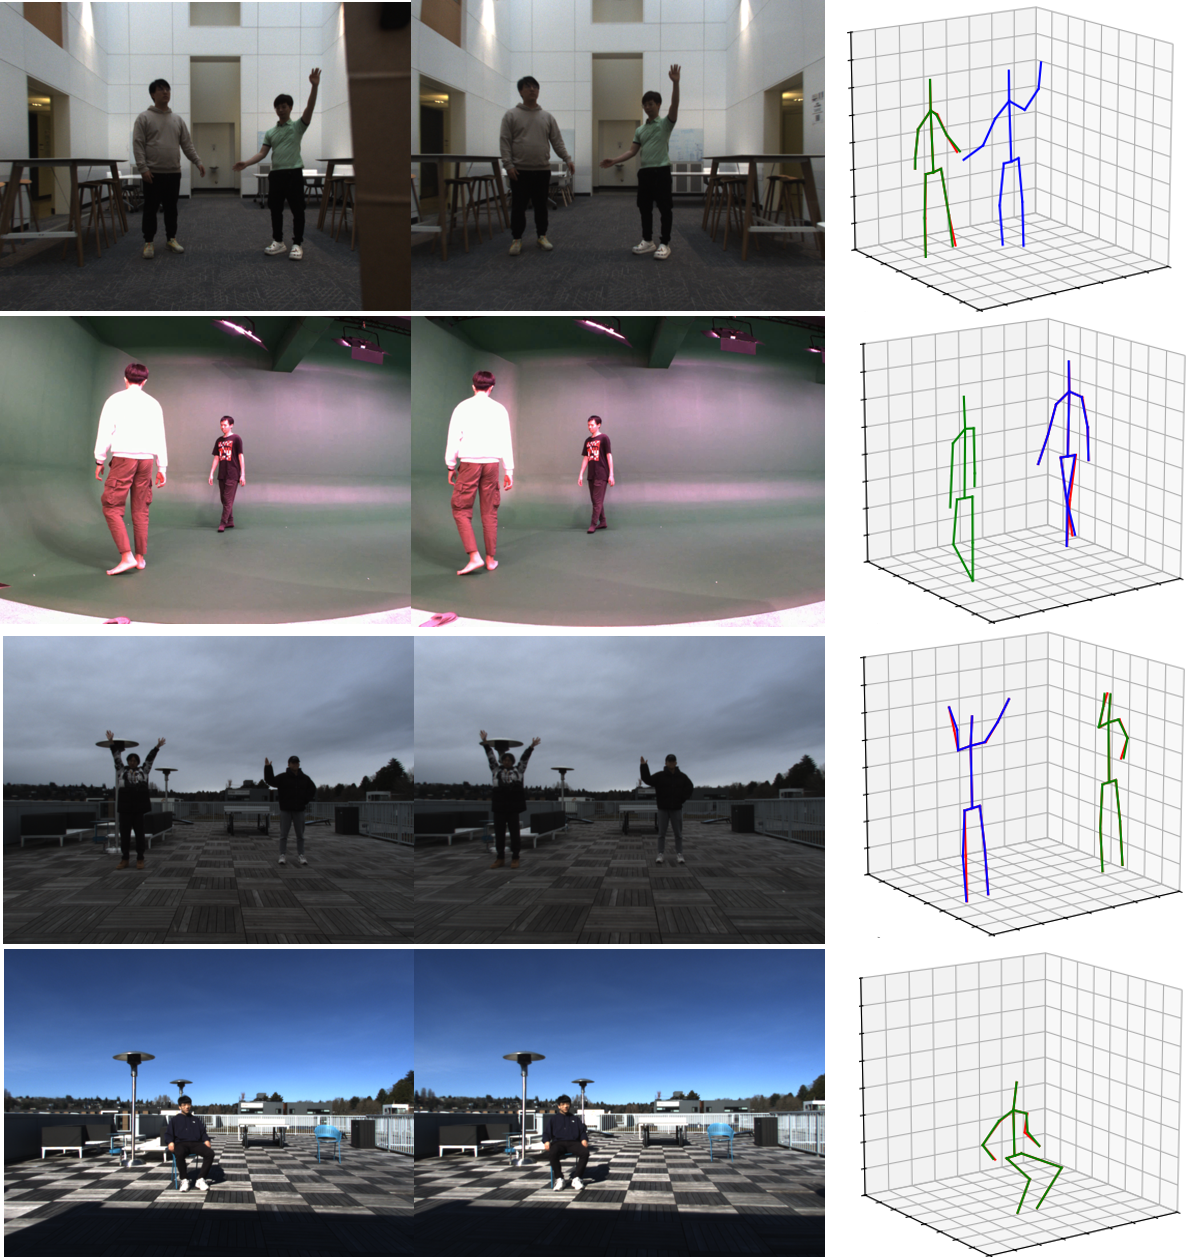
\includegraphics[width=0.8\linewidth]{../figures/visual-result-2.png}
\centering
\caption{Qualitative results of our method on the RT-Pose dataset. Red skeletons indicate ground-truth poses, while distinct colors represent our model's predictions for different subjects. } \label{fig4}
\end{figure}
We present qualitative results to visually demonstrate the effectiveness of our proposed method in recovering accurate 3D human poses. As shown in Fig.~\ref{fig3}, StereoMulti3DPose produces reliable and consistent 3D pose estimations across multi-person scenarios and a variety of complex human actions.

\begin{figure}[!h]

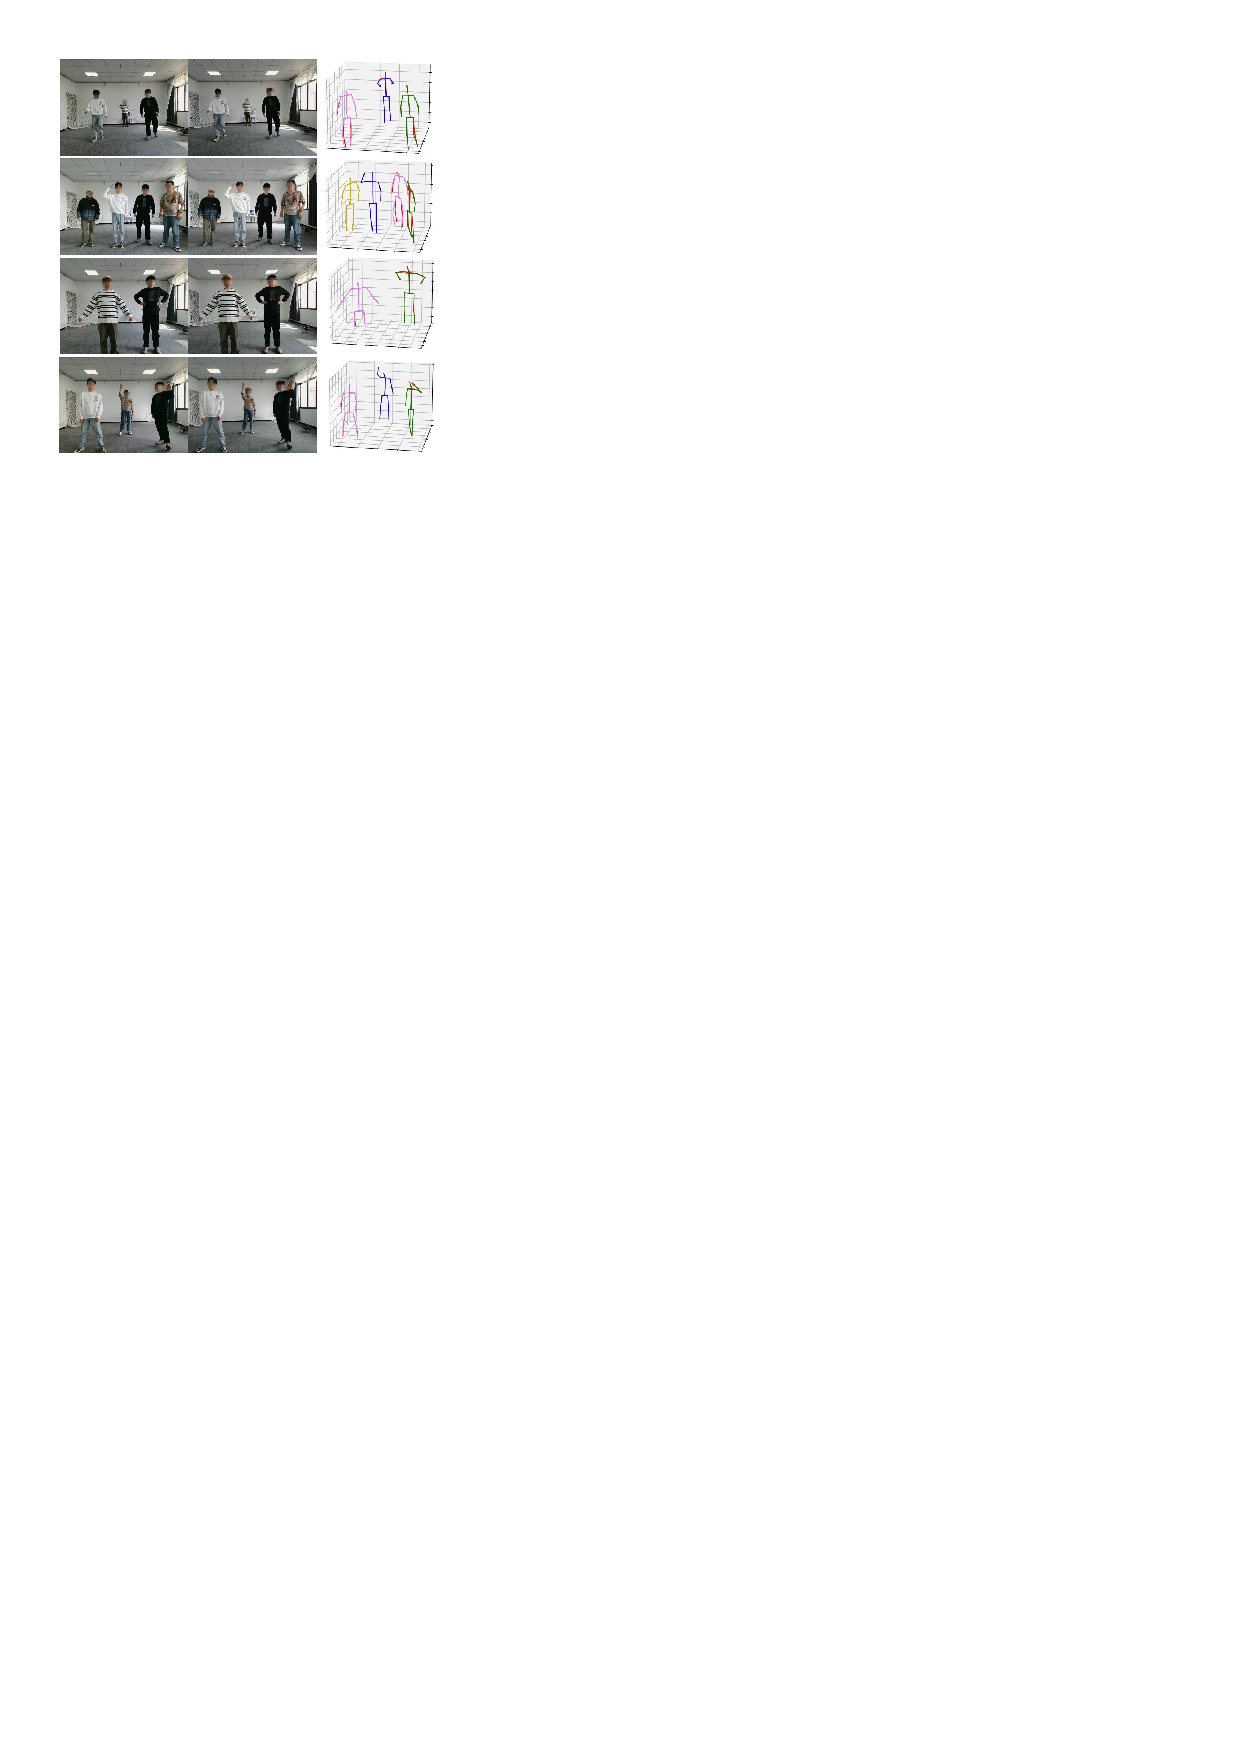
\includegraphics[width=0.8\linewidth]{../figures/visualx4.pdf}
\centering
\caption{Qualitative results of our method on the BMP dataset. Red skeletons indicate ground-truth poses, while distinct colors represent our model's predictions for different subjects. } \label{fig3}
\end{figure}





\subsection{Ablation Study}

\textbf{Performance Impact of EFEM} To evaluate the impact of the Epipolar Feature Enhancement Module (EFEM) on model accuracy, we conducted a series of ablation studies. First, we assessed the model's performance after removing EFEM entirely. Then, we replaced EFEM with simple concatenation and a 1×1 convolution to analyze its effect on accuracy. For a fair comparison, we maintained the distillation strategy across all experiments. As shown in Table~\ref{The Importance of EFEM}, removing EFEM led to a significant drop in accuracy. Compared to concatenation and 1×1 convolution, EFEM demonstrated a superior ability to capture feature differences.

\begin{table}[!h]
\centering
\caption{Comparison of the impact of different feature enhancement modules in dual-branch models.}
\renewcommand{\arraystretch}{1.1}
\small
\label{The Importance of EFEM}
\begin{tabular}{l|cc}
\hline
\textbf{Feature Enhancement Module} & \textbf{MPJPE (mm) $\downarrow$}\\
\hline
None & 120.4 \\
Concat + Conv1x1 \citess{he2020epipolar} &   72.3 \\
EFEM   &  \textbf{51.0} \\
\hline
\end{tabular}
\end{table}

\begin{table}[!htbp]
\centering
\caption{Comparison of different methods for pose and depth refinement}
\renewcommand{\arraystretch}{1.1}
\small
\label{The Importance of PoseDepth Refinement Module}
\begin{tabular}{l|cc}
\hline
\textbf{Methods} &  \textbf{MPJPE (mm) $\downarrow$}\\
\hline
2D Keypoint Matching \citess{niemirepo2020binocular}  & 89.3 \\
Depth Regression \citess{sun2018integral} &   72.4 \\
PDRM  &  \textbf{51.0} \\

\hline
\end{tabular}
\end{table}


\textbf{Performance Impact of  PDRM}
To evaluate the effectiveness of the proposed PoseDepth Refinement Module (PDRM), we compared it against two simplified baselines: (1) depth estimation via 2D keypoint matching and (2) direct depth regression without prior initialization. As shown in Table~\ref{The Importance of PoseDepth Refinement Module}, 2D keypoint matching yields an MPJPE of 89.3 mm due to limited sub-pixel precision and sensitivity to disparity noise. Depth regression improves accuracy (72.4 mm) by learning geometric priors, but lacks stable initialization. In contrast, PDRM achieves the lowest MPJPE of 51.0 mm by combining coarse triangulation with fine-grained refinement, reducing errors by up to 43\% compared to keypoint matching. This demonstrates the benefit of our constrained, two-stage depth estimation strategy.



\textbf{Performance Impact of  Feature Distillation}
To investigate the effectiveness of distillation in enhancing the feature extraction capability of the lightweight branch, we conducted an ablation study by disabling the distillation module during training for comparison. As shown in Table~\ref{The Importance of Distillation}, applying distillation to either the backbone or neck leads to clear performance gains, while combining both yields the best result, reducing MPJPE from 92.3 to 51.0. This suggests that backbone and neck distillation provide complementary benefits, and jointly improving low- and high-level features significantly enhances the lightweight branch’s representation ability.


To justify the selection of MSE loss with 1$\times$1 convolutions for feature alignment, we conducted a comparative experiment against KL divergence and Cosine Similarity. As shown in Table \ref{distillation_loss}, our MSE-based strategy yields a 44.7\% reduction in MPJPE compared to the non-distilled baseline, significantly outperforming other alignment methods.


The superiority of this approach stems from the fundamental nature of the task and our asymmetric architecture. First, while KL divergence is optimized for aligning discrete probability distributions (e.g., logits), our distillation occurs at the intermediate feature level, where neurons represent continuous geometric activations that require precise intensity regression. Second, unlike Cosine Similarity which only accounts for vector orientation, MSE enforces alignment in both direction and magnitude; the latter is critical for encoding the matching confidence and spatial cues required by the subsequent PDRM module to mitigate stereo uncertainty. Finally, the 1$\times$1 convolution acts as a learnable projection layer that maps the disparate channel dimensions of the full-scale and lightweight branches into a consistent manifold, ensuring that the student branch effectively inherits high-quality representations from the teacher without losing discriminative power.

\begin{table}[htbp]
\centering
\caption{Comparison of different distillation loss functions on the BMP dataset. Our MSE-based alignment achieves the highest error reduction.}
\label{distillation_loss}
\renewcommand{\arraystretch}{1.1}
\small
\begin{tabular}{l|c|c}
\hline
\textbf{Distillation Strategy} & \textbf{MPJPE (mm) $\downarrow$} & \textbf{Improv. (\%)} \\ \hline
None (Baseline)                & 92.3                             & -                         \\
KL Divergence                  & 78.4                             & 15.1\%                    \\
Cosine Similarity              & 71.2                             & 22.8\%                    \\
\textbf{1$\times$1 Conv + MSE (Ours)} & \textbf{51.0}             & \textbf{44.7\%}           \\ \hline
\end{tabular}
\end{table}


\textbf{Performance Impact of Depth Hyper-parameter}
To examine the effect of $\Delta D$ on model accuracy, we varied its value from 5 cm to 50 cm, and the results are reported in Table~\ref{The Importance of D}. A larger $\Delta D$ enlarges the search space, allowing more candidate solutions to be considered, but at the cost of reduced efficiency and increased noise. In contrast, a smaller $\Delta D$ enables more precise estimation but limits the search to a narrow local region, potentially missing superior solutions.
\begin{table}[h]
\centering
\caption{Ablation study on the effect of distillation at different stages.}
\renewcommand{\arraystretch}{1.1}
\small
\label{The Importance of Distillation}
\begin{tabular}{l|c}
\hline
\textbf{Distillation Setting} & \textbf{MPJPE (mm) $\downarrow$} \\
\hline
None & 92.3 \\
Backbone only & 78.9 \\
Neck only & 63.3 \\
Backbone + Neck & \textbf{51.0} \\
\hline
\end{tabular}
\end{table}
\begin{table}[!htb]
\centering
\caption{Ablation study on the selection of hyperparameters $\Delta D$ }
\renewcommand{\arraystretch}{1.1}
\small
\label{The Importance of D}
\begin{tabular}{c|ccccc}
\hline
\textbf{$\Delta D$} &  5cm &  10cm  &  20cm &  30cm &  50cm\\
\hline
\textbf{MPJPE} & 126.5  & 77.9 & \textbf{51.0} & 68.3 & 84.4\\

\hline
\end{tabular}
\end{table}

To justify the discretization of the depth search space in PDRM, we analyzed the impact of different bin counts ($K$) on accuracy and inference latency. We fixed the search range $\Delta D=20$ cm (total 40 cm span) and varied $K$ from 64 to 512. The results are presented in Table~\ref{tab:bin_ablation}. As shown in the table, increasing the bin count from 64 to 128 yields a significant 26.5 mm improvement in MPJPE, as 128 bins provide a fine-grained spatial resolution of approximately 3.1 mm per bin. However, further increasing $K$ to 256 results in diminishing returns (0.8 mm gain), as the resolution (1.5 mm) begins to approach the inherent precision limit of sparse pixel-level keypoint detectors. Notably, when $K$ is further increased to 512, the accuracy actually degrades (MPJPE increases to 69.5 mm). This is because a sub-millimeter resolution (0.78 mm) far exceeds the effective information provided by lightweight detectors; in this regime, the module begins to model detection noise rather than valid geometric signals. Furthermore, an excessively large $K$ increases the sparsity of the label space, making the classification-based Softmax distribution harder to optimize. Regarding efficiency, although the latency increases with $K$, the 3D head still accounts for only $\approx$1\% of the total inference time. Thus, $K=128$ is chosen as the optimal balance between 3D localization precision and model convergence stability.

\begin{table}[htbp]
    \centering
    \caption{Ablation study on the bin count $K$ in the PDRM module (evaluated on the BMP dataset).}
    \label{tab:bin_ablation}
    \renewcommand{\arraystretch}{1.3}
    \setlength{\tabcolsep}{4pt}
    \resizebox{\columnwidth}{!}{
        \begin{tabular}{l|ccc}
            \hline
            \textbf{Bin Count ($K$)} & \textbf{Resolution (mm)} & \textbf{MPJPE (mm) $\downarrow$} & \textbf{Latency (ms)} \\ \hline
            64                       & 6.25                     & 77.5                             & 115.2                 \\ \hline
            \textbf{128 (Ours)}      & \textbf{3.12}            & 51.0                  & \textbf{116.0}        \\ \hline
            256                      & 1.56                     & \textbf{50.2}                             & 120.4                 \\ \hline
            512                      & 0.78                     & 69.5                             & 126.0                 \\ \hline
        \end{tabular}
    }
\end{table}


\textbf{Performance Impact of Loss Weight Ratios}
To investigate the influence of loss weights on StereoMulti3DPose, we evaluate the \textit{Effective Weight Ratio}, defined as $(\lambda_1 + \lambda_2) : \lambda_3$. This ratio balances primary task supervision ($\lambda_1$ for XY-plane and $\lambda_2$ for Z-axis) against teacher-guided geometric distillation ($\lambda_3$). In our implementation, we maintain a fixed internal ratio of $\lambda_1 : \lambda_2 = 1:1$ to ensure the model places equal emphasis on planar precision and depth consistency.

As detailed in Table~\ref{tab:ablation_lambda3}, Table~\ref{tab:ablation_lambda12} and Fig. \ref{u_shape}, we conducted two independent experimental sets: (1) fixing the primary task weight sum at 10 while varying $\lambda_3$, and (2) fixing $\lambda_3 = 1$ while varying the task weights. Despite the different tuning strategies, both sets converge to a consistent U-shaped trajectory, reaching a global optimal MPJPE of 51.0 mm at the 10:1 ratio. When $\lambda_3$ is negligible (e.g., 1000:1 ratio), the lightweight student branch lacks sufficient geometric priors, causing performance to degrade toward the 86.4 mm. As the ratio approaches 1:1 ($\lambda_3 = 10$), the MPJPE collapses to 105.4 mm. This occurs because excessive distillation forces the student network to overfit the teacher's intermediate representations, suppressing the learning of core coordinate signals.

The convergence of both experimental paths at the 10:1 point confirms that the relative ratio, rather than absolute weight values, dictates the system's physical equilibrium.
\begin{figure}[hp]
    \centering
    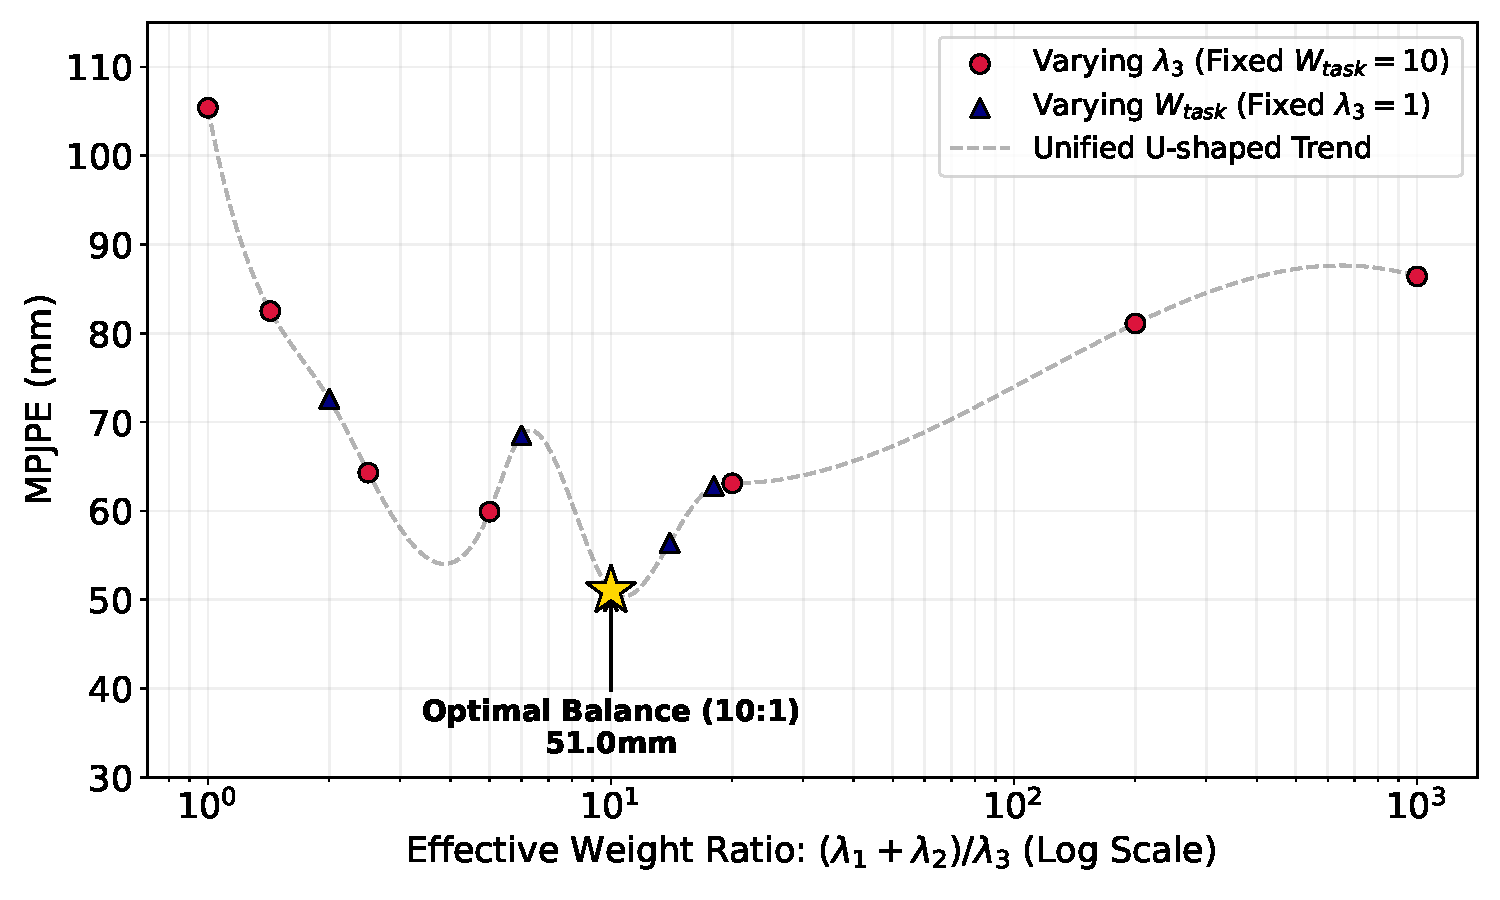
\includegraphics[width=\linewidth]{../figures/lossR.pdf}
    \caption{MPJPE Sensitivity Analysis. The figure illustrates the MPJPE evolution across varying weight ratios using a logarithmic scale for the x-axis. Data points from \textit{Set 1} (varying $\lambda_3$) and \textit{Set 2} (varying $\lambda_{1,2}$) are fitted to a single U-shaped curve. The curve reveals that the system reaches its physical equilibrium at a 10:1 ratio, while accuracy suffers from insufficient guidance at high ratios and task interference at low ratios.}
    \label{u_shape}
\end{figure}


\begin{table}[h]
\centering
\caption{Ablation study on hyperparameter $\lambda_3$ (with fixed $\lambda_{1} = \lambda_{2} = 5$)}
\renewcommand{\arraystretch}{1.1}
\small
\label{tab:ablation_lambda3}
\renewcommand{\arraystretch}{1.2}
\setlength{\tabcolsep}{4pt}
\begin{tabular}{c|cccccccc}
\hline
$\lambda_{3}$ & 0.01 & 0.05 & 0.5 & 1 & 2 & 4 & 7 & 10 \\ \hline
\textbf{MPJPE} $\downarrow$ & 86.4 & 81.1 & 63.1 & \textbf{51.0} & 59.9 & 64.3 & 82.5 & 105.4 \\ \hline
\end{tabular}
\end{table}

\begin{table}[ht]
\centering
\caption{Ablation study on hyperparameters $\lambda_{1}, \lambda_{2}$ (with fixed $\lambda_{3} = 1$)}
\renewcommand{\arraystretch}{1.1}
\small
\label{tab:ablation_lambda12}
\renewcommand{\arraystretch}{1.2}
\setlength{\tabcolsep}{8pt}
\begin{tabular}{l|ccccc}
\hline
$\lambda_{1}=\lambda_{2}$ & 1 & 3 & 5 & 7 & 9 \\ \hline
\textbf{MPJPE} $\downarrow$ & 72.6 & 68.5 & \textbf{51.0} & 56.4 & 62.8 \\ \hline
\end{tabular}
\end{table}

\textbf{Performance Impact of Asymmetric Architecture and Backbone Generality} To demonstrate that our proposed framework is a general 3D perception paradigm independent of specific backbones, we evaluate its performance under various architectural configurations.


\begin{table*}[ht]
\centering
\caption{Comprehensive ablation study and generality analysis of \textit{StereoMulti3DPose}. We evaluate the impact of the asymmetric dual-branch paradigm, geometric modules, and distillation across various backbones. Note: All "Asymmetric" and "Generality" configurations implicitly include the PDRM module. \textbf{Symmetric (Full)} includes distillation to maintain a unique variable (student scale) for comparison with our proposed model.}
\label{backbone_generality}
\renewcommand{\arraystretch}{1.2}
\begin{tabular}{llccccccc}
\hline
\textbf{Category} & \textbf{Left (Teacher)} & \textbf{Right (Student)} & \textbf{EFEM} & \textbf{Distill} & \textbf{MPJPE (mm)} $\downarrow$ & \textbf{FLOPs (G)} $\downarrow$ & \textbf{Latency (ms)} $\downarrow$ \\ \hline

Symmetric (Light) & ShuffleNetV2 \citess{ma2018shufflenet}& ShuffleNetV2 & - & - & 120.4 & 13.41 & 108.2 \\
Symmetric (Full) & CSPDarknet & CSPDarknet & \checkmark & \checkmark & 49.5 & 27.18 & 215.4 \\ \hline
Asymmetric Base & CSPDarknet & ShuffleNetV2 & - & - & 92.3 & 13.59 & 110.5 \\
Asymmetric + EFEM & CSPDarknet & ShuffleNetV2 & \checkmark & - & 72.3 & 13.75 & 113.2 \\
\textbf{Proposed (Ours)} & \textbf{CSPDarknet} & \textbf{ShuffleNetV2} & \checkmark & \checkmark & \textbf{51.0} & \textbf{13.93} & \textbf{116.0} \\ \hline

Generality Group 1 & EfficientNet-B0 \citess{tan2019efficientnet} & MobileNetV3-S \citess{koonce2021mobilenetv3}& \checkmark & - & 85.6 & 12.15 & 105.4 \\
& EfficientNet-B0   & MobileNetV3-S  & \checkmark & \checkmark & 54.2 & 12.15 & 105.4 \\ \hline
Generality Group 2 & ResNet-50 \citess{he2016deep}& ShuffleNetV2 & \checkmark & - & 78.4 & 22.40 & 168.2 \\
& ResNet-50 & ShuffleNetV2 & \checkmark & \checkmark & 49.8 & 22.40 & 168.2 \\ \hline

Generality Group 3 & CSPDarknet & \textbf{GhostNet (x1.0)}\citess{Han_2020_CVPR} & \checkmark & - & 79.5 & 13.90G & 119.5ms \\
             & CSPDarknet & \textbf{GhostNet (x1.0)}  & \checkmark & \checkmark & \textbf{52.8} & 13.90G & 119.5ms \\ \hline
\end{tabular}
\end{table*}

To validate the effectiveness of the core components in StereoMulti3DPose and their generalizability across various architectures, we conducted a comprehensive ablation and generality study (Table \ref{backbone_generality}). Experimental results demonstrate that compared to the traditional symmetric architecture (Symmetric Full), our asymmetric dual-branch paradigm achieves an optimal balance between accuracy and efficiency. Specifically, it reduces FLOPs by 48.7\% (from 27.18G to 13.93G) and slashes inference latency by 46.1\% (from 215.4ms to 116.0ms) with a marginal precision loss of only 1.5 mm.
The ablation analysis reveals the individual contributions of our proposed modules. The Epipolar Feature Enhancement Module (EFEM) provides a crucial geometric boost by capturing cross-view discrepancies along horizontal epipolar lines, significantly reducing the MPJPE from 92.3 mm to 72.3 mm. Furthermore, our online feature distillation strategy enables the lightweight right branch to align its representations with the high-fidelity features of the left branch. This "zero-cost" optimization further suppresses the error to 51.0 mm without imposing any additional computational burden during inference.
Moreover, the Generality Groups (1-3) demonstrate the framework’s robust adaptability across diverse IoT backbones. Whether utilizing heavy-duty (ResNet-50 \citess{he2016deep}) or ultra-lightweight (GhostNet\citess{Han_2020_CVPR}, MobileNetV3 \citess{tan2019efficientnet}) student branches, the distillation strategy consistently delivers an accuracy improvement exceeding 30\%.


\textbf{Robustness to Rectification Errors}
To evaluate the sensitivity to imperfect rectification (e.g., caused by thermal drift or vibrations), we manually introduced vertical pixel offsets during inference. As shown in Table ~\ref{rectification_error}, StereoMulti3DPose demonstrates high resilience: a 2-pixel vertical error only results in a 3.5\% increase in MPJPE. This robustness is attributed to: 1) the coarse 1/16 scale of EFEM, where preceding receptive fields absorb minor spatial displacements; and 2) the probabilistic PDRM, which mitigates matching uncertainties through expectation-based depth recovery rather than rigid geometric triangulation.

\begin{table}[htbp]
\centering
\caption{Sensitivity of MPJPE to vertical rectification errors.}
\label{rectification_error}
\renewcommand{\arraystretch}{1.1}
\small
\begin{tabular}{l|cccc}
\hline
\textbf{Vertical Offset} & \textbf{0 (Base)} & \textbf{1 px} & \textbf{2 px} & \textbf{5 px} \\ \hline
MPJPE (mm)               & 51.0              & 51.4          & 52.8          & 58.6          \\
Degradation (\%)         & -                 & 0.8\%         & 3.5\%         & 14.9\%        \\ \hline
\end{tabular}
\end{table}



\textbf{View-Invariance Robustness Analysis} A potential concern with the asymmetric dual-branch design is the introduction of view-dependent bias, where the model might become overly reliant on the full-scale left branch (i.e., becoming "left-handed"). To assess this, we conducted a Swapping Test during inference, where the left and right images were interchanged before being fed into the fixed heavy and light branches.

As shown in Table \ref{tab:swap_test}, when the input views are swapped, the MPJPE only increases slightly from 51.0 mm to 52.1 mm (a marginal gap of 2.1\%). This robustness confirms that our symmetric training strategy effectively decouples the geometric perception from the specific backbone scale. By training the network to be indifferent to which branch receives the primary viewpoint, the EFEM successfully masters the underlying epipolar geometry, ensuring stable performance regardless of the input configuration.

\begin{table}[htbp]
\centering
\caption{Robustness test against view-dependent bias via input swapping.}
\label{tab:swap_test}
\begin{tabular}{@{}lcc@{}}

\hline
\textbf{Input Configuration} & \textbf{MPJPE (mm)} & \textbf{Performance Gap} \\
\hline
(Left $\to$ Full, Right $\to$ Comp.) & 51.0 & - \\
\hline
(Right $\to$ Full, Left $\to$ Comp.) & 52.1 & +2.1\% \\
\hline
\end{tabular}
\end{table}

\textbf{Performance Impact of Two-Stage Training Strategy}

We evaluated our training strategy against various paradigms as shown in Table \ref{tab:training_strategy_ablation}. While Synthetic Only (92.5 mm) and Real Only (71.2 mm) configurations struggled with sensor noise and overfitting respectively, joint training on mixed data proved suboptimal (54.8 mm) due to domain interference, where disparate pixel distributions caused gradient conflicts. In contrast, our two-stage curriculum learning first internalizes stable epipolar geometric priors from 100k synthetic pairs via distillation, then adapts to real-world complexities through fine-tuning on the BMP dataset. This sequential approach successfully bridges the sim-to-real gap, achieving a superior 51.0 mm MPJPE by prioritizing fundamental physical laws before environmental details.
\begin{table}[h]
\centering
\caption{Ablation study of training strategies on the BMP real-world test set. The results highlight the superiority of the two-stage "Synthetic $\rightarrow$ Real" paradigm over joint training.}
\label{tab:training_strategy_ablation}
\renewcommand{\arraystretch}{1.2}
\begin{tabular}{llc}
\hline
\textbf{Training Strategy} & \textbf{Dataset Configuration} & \textbf{MPJPE (mm)} $\downarrow$ \\ \hline
Synthetic Only & SSMP (100k) & 92.5 \\
Real Only & BMP (20k) & 71.2 \\
Joint Training & SSMP + BMP (Mixed) & 54.8 \\
\textbf{Two-stage (Ours)} & \textbf{SSMP $\rightarrow$ BMP} & \textbf{51.0} \\ \hline
\end{tabular}
\end{table}
\section{Discussion}

In this section, we further elaborate on several design choices and potential extensions of StereoMulti3DPose to address the feedback regarding deployment efficiency, robustness, and architectural specialization.

Regarding the training strategy and dynamic adaptation, while test-time distillation or online adaptation could theoretically improve deployment accuracy, they pose significant challenges for resource-constrained IoT nodes. Our framework is designed to deliver a fixed real-time latency of 116 ms on platforms like the Xiaomi 14 (Snapdragon 8 Gen3), ensuring computational stability in time-sensitive robotics and monitoring applications. Introducing test-time backpropagation or online weight updates would compromise this deterministic performance and significantly increase power consumption, which is critical for battery-operated edge devices. Similarly, although dynamic pruning or scaling of the student branch based on scene complexity could reduce FLOPs in simple environments, the "on-the-fly" overhead of dynamic re-configuration often offsets the energy gains and introduces non-deterministic execution paths that are difficult to optimize with fixed-function NPU toolchains.

Occlusion handling remains a pivotal challenge in 3D multi-person pose estimation as binocular systems are inherently restricted by the physical limitations of dual-view observation. StereoMulti3DPose mitigates this issue via the PDRM, which replaces traditional direct regression with a discrete probability distribution over quantized bins to effectively manage geometric uncertainty. However, as shown in our qualitative analysis, information loss during severe body-on-body occlusion can still lead to keypoint drift. Fundamentally resolving such cases may necessitate multi-view systems or the integration of temporal aggregation and graph-based relational modeling to enhance keypoint recovery in dense environments.

Regarding the architectural choice of the PDRM, the use of MLPs instead of convolutional decoders is a deliberate decision based on the sparsity of the input features. Unlike dense stereo matching which requires 3D or 2D convolutions to aggregate spatial contexts over a grid, the PDRM operates on sparse, joint-aware feature vectors extracted from detected person instances. Utilizing convolutional decoders for such sparse representations would impose an unnecessary computational burden, contradicting our goal of keeping the refinement stage at approximately 1\% of the total inference time. MLPs effectively capture the cross-view correspondence within the narrow disparity search range ($\pm$20 cm) while maintaining the lightweight footprint required for IoT deployment.

The superior efficiency of the Epipolar Feature Enhancement Module (EFEM) is rooted in its geometric intelligence rather than computational brute force. While adding a negligible 1.5 MB of parameters (less than 13\% of the total model size), EFEM delivers a substantial 29\% improvement in MPJPE compared to simple concatenation-based fusion. This high parameter efficiency is achieved by constraining the cross-view attention mechanism to the horizontal epipolar lines of rectified stereo pairs. Unlike general multi-view transformers that incur heavy costs through global attention, EFEM reduces the search space to a 1D trajectory, effectively filtering out geometric noise and enabling the lightweight branch to capture high-fidelity spatial cues from the full-scale branch. Furthermore, whereas traditional two-stage methods rely on computationally heavy 3D cost volumes for dense matching, our EFEM operates on sparse, high-level semantic features. By modeling the physical law of binocular vision—where corresponding points must lie on the same scanline—the EFEM transforms a generic feature extraction process into a geometry-driven reasoning engine, ensuring robust 3D localization even within the strict FLOPs budget of IoT edge devices.

Finally, we address the use of the RT-Pose dataset and the choice of sensing modalities. While RT-Pose provides LiDAR and radar data, our framework intentionally utilizes only stereo RGB images. This aligns with our objective to design a solution for widely available IoT hardware, such as mobile devices and low-power embedded perception modules, which rarely feature expensive LiDAR or high-bandwidth radar sensors. By demonstrating state-of-the-art accuracy (158.6 mm MPJPE) using only stereo cameras, we highlight the framework's portability and practical deployment potential across diverse edge computing ecosystems without requiring complex multi-sensor synchronization.

\section{Conclusions  and Future Works}




In this paper, we presented StereoMulti3DPose, a lightweight stereo-based 3D multi-person pose estimation framework specifically engineered for the unique constraints of IoT devices. Our research bridges the critical gap between server-level 3D perception and the low-power requirements of edge hardware. By designing an asymmetric dual-branch architecture and integrating geometry-aware modules like EFEM and PDRM, we have demonstrated that explicit geometric priors can effectively substitute for raw model capacity. This allows our framework to achieve high-precision results (51.0 mm MPJPE) while reducing computational redundancy by 43\% compared to symmetric dual-branch baselines.

The significance of our findings lies in the realization that sophisticated 3D human understanding no longer necessitates high-end GPUs or complex multi-camera arrays. Our study offers a key insight: through online feature distillation, a lightweight student network can internalize complex epipolar laws from a high-capacity teacher branch during training, thereby maintaining geometric consistency without any added inference overhead. Furthermore, the achieved deterministic latency of 116 ms on mobile platforms (e.g., Snapdragon 8 Gen3) proves that real-time 3D pose estimation is now a genuinely deployable technology for time-critical IoT ecosystems.

The practical applicability of StereoMulti3DPose extends to a wide range of privacy-sensitive and bandwidth-limited scenarios, including real-time healthcare monitoring, human–robot collaboration, and autonomous smart home surveillance. By enabling on-device processing, our framework ensures user data security and operational resilience in disconnected environments, eliminating the need for risky cloud offloading.

Looking forward, although our method achieves state-of-the-art efficiency, physical limitations of dual-view observation still pose challenges under severe body-on-body occlusion. In future work, we plan to integrate temporal aggregation and graph-based relational modeling to further enhance the recovery of missing keypoints. These advancements, combined with hardware-aware model compression and NNAPI/ASIC-oriented optimization, will continue to drive the evolution of intelligent, autonomous edge nodes capable of sophisticated, privacy-friendly human understanding.

\bibliographystyle{IEEEtran}
\bibliography{refs}


\vspace{-1.3cm}
\begin{IEEEbiography}[{
\includegraphics[width=1in,height=1in,clip,keepaspectratio]{../authors/DeyuZhang.png}}]{Deyu Zhang}
	is an associate professor in School of Computer Science and Technology at Central South
	University. He received the B.Sc. degree in communication engineering from PLA Information Engineering University, Zhengzhou, China, in 2005, and the M.Sc. degree in communication engineering and Ph.D. degree in computer science from Central South University, Changsha, China, in 2012 and 2016, respectively. His current research interests include mobile system optimization, edge computing, and stochastic optimization.
\end{IEEEbiography}

\vspace{-1.5cm}
\begin{IEEEbiography}[{
\includegraphics[width=1in,height=1in,clip,keepaspectratio]{../authors/wkq.jpg}}]{\\Kangqi Wei}
	received the B.Sc. degree in 2023 from the School of Computer Science and Engineering, Hefei University of Technology, XuanCheng, China. Now he is a postgraduate student in the School of Computer Science at Central South University. His research interests include computer vision, edge computing, and heterogeneous computing.
\end{IEEEbiography}


\vspace{-1.5cm}
\begin{IEEEbiography}[{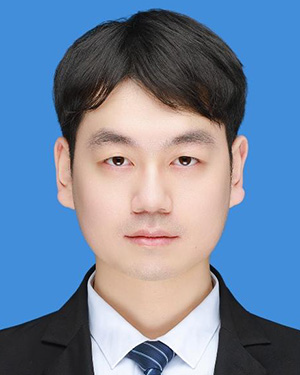
\includegraphics[width=1in,height=1in,clip,keepaspectratio]{../authors/yanghuan.png}}]{\\Huan Yang} received the
B.Sc. degree from the College of Mathematics
and Computer Science, Fuzhou University, Fuzhou,
China, in 2021. He received the M.S. degree from Central South University, Changsha,
China, in 2023. He is currently pursuing the Ph.D. degree with Central South University, Changsha, China. His research interests include large language model, heterogeneous computing and edge computing.
\end{IEEEbiography}

\vspace{-1.5cm}
\begin{IEEEbiography}[{
\includegraphics[width=1in,height=1in,clip,keepaspectratio]{../authors/tangyin.jpg}}]{\\Yin Tang}
received the M.S. degree from Nanjing Normal University, Nanjing, Jiangsu, China, in 2022. He is currently pursuing the Ph.D. degree with Central South University, Changsha, China. His research interests include video understanding, action recognition, heterogeneous computing and edge computing.
\end{IEEEbiography}

\vspace{-1.5cm}
\begin{IEEEbiography}[{
\includegraphics[width=1in,height=1in,clip,keepaspectratio]{../authors/Fan_Wu.pdf}}]{\\Fan Wu}
received his Ph.D. degree in Computer Science and Technology from Central South University, Changsha, China in 2020.
During 2018-2019, he was a visiting Ph.D. student in BBCR Group, Department of Electrical and Computer Engineering, University of Waterloo, Canada.
He worked as a Postdoctoral Fellow with the Department of Computer Science and Technology, Tsinghua University, from Jul. 2020 to Nov. 2022.
Dr. Wu is currently an assistant professor with the School of Computer Science and Engineering, Central South University.
His current research interests include Internet of Things, mobile edge computing, data mining, and big data.
\end{IEEEbiography}

\end{document}




































































































